%% ===========================================================================
%%  The Price of Stale State: When Does Network Awareness Pay in LLM Inference
%%  Serving?
%%
%%  编译：latexmk -pdf main.tex    （或 pdflatex main && bibtex main && pdflatex main ×2）
%%
%%  【模板说明】这里用 IEEEtran 的 journal 模式——它自包含、TeX Live/MiKTeX 都带，
%%  投稿 IEEE 系期刊（TPDS/ToN 等）或多数 SCI 期刊时可直接用。
%%  若改投 Elsevier（如 Computer Networks），把 documentclass 换成
%%      \documentclass[preprint,12pt]{elsarticle}
%%  并把 \begin{abstract}...\end{abstract} 之外极少量的命令替换即可，正文不用动。
%%
%%  【数字来源】正文里**每一个数字**都来自 `sim/results/paper_numbers.txt`，
%%  该文件由 `sim/analysis/export_paper_numbers.py` 从三批分析产物自动导出。
%%  改数字前请先改产物、再改正文，禁止手改正文里的数。
%% ===========================================================================
\documentclass[journal,10pt]{IEEEtran}

\usepackage{graphicx}
\usepackage{booktabs}
\usepackage{amsmath,amssymb}
\usepackage{url}
\usepackage{xcolor}
\usepackage{array}
\usepackage{multirow}
\usepackage{siunitx}
\usepackage[hidelinks]{hyperref}

\graphicspath{{figures/}}
\DeclareGraphicsExtensions{.pdf,.png,.jpg}

% 允许排版器在必要时多拉伸一点词间距，避免长引用组（\cite{a,b,c}）与长标识符
% 冲出栏宽（overfull \hbox）。比手改每一句更省事，且对英文正文观感无影响。
\setlength{\emergencystretch}{3em}

% 让表格里的数字列更紧凑
\newcolumntype{R}[1]{>{\raggedleft\arraybackslash}p{#1}}

\begin{document}

\title{The Price of Stale State: When Does Network Awareness Pay in \\
       LLM Inference Serving?}

% ===========================================================================
%  ★★★ 署名：投稿前必须替换这一块 ★★★
%  下面 `\author{...}` 里是**占位符**，请把方括号里的内容换成你自己的信息：
%      [Author Name]   → 你的姓名（英文拼写，如 "San Zhang"）
%      [Affiliation]   → 单位（如 "School of Computer Science, XX University"）
%      [City]/[Country]、[email@example.org]
%  若是**双盲评审**（要求隐去作者），把它换回：
%      \author{\IEEEauthorblockN{Anonymous Authors}\IEEEauthorblockA{Authors and
%      affiliations withheld for review.}}
%  多数期刊的终稿还要求：通讯作者标记 \thanks{Corresponding author: ...}、
%  基金号 \thanks{This work was supported by ...}、以及每位作者的简介与照片。
% ===========================================================================
\author{%
\IEEEauthorblockN{[Author Name]}
% 注意 `\\{}`：`\\` 后面直接跟 `[` 会被 LaTeX 当成长度参数（Missing number 报错），
% 加一个空的 `{}` 就切断了这种解析。踩过一次。
\IEEEauthorblockA{[Affiliation], [City], [Country]\\{}
                  [email@example.org]}}

\maketitle

\begin{abstract}
Network-aware request scheduling for LLM inference---routing each request to the worker
jointly best in compute backlog and link state---is widely reported to improve tail latency, yet
reported gains range from negligible to over 70\%, and one published system reports that its gains
persist under telemetry delayed by \SI{60}{\second}. We ask the prior question: \textbf{when does
network awareness pay, and when does trusting it hurt?} Using a discrete-event simulator with up to
ten independent workload realizations per cell across three sources (synthetic, the Azure LLM
trace, and BurstGPT), plus a real single-node \texttt{k3s} cluster, we report four findings.
(1)~Under our controlled configurations, the benefit tracks compute--bandwidth rank
disagreement more than link speed: it is $-3.3\%$ when the
fastest-computing worker also has the widest link and $-68.2\%$ when the two rankings disagree
(Cliff's $\delta=1.00$, $p=1.8\times10^{-4}$), persisting at 4, 8 and 16 workers.
(2)~The two observed channels expire an order of magnitude apart: queue state loses $56$--$85\%$ of
its value within \SI{5}{\second}, while link state retains $65$--$89\%$ at \SI{60}{\second}. This
explains the published ``\SI{60}{\second} does not matter'' observation, which swept only the
slow-expiring channel. (3)~Per-channel discounting retains $90$--$99\%$ of the benefit under
\SI{60}{\second}-old link state, where uniform discounting destroys all of it; our own first
design is falsified by our own experiments. (4)~On real containers, a state read costs
\SIrange{56}{876}{\milli\second} against \SI{12}{\micro\second} for an in-cluster round trip,
grows with load, and staleness hurts in a threshold-like manner. We also report what did
\emph{not} work, including two refuted hypotheses. We additionally report a \emph{descriptive}
two-cloud deployment anchor: bidirectional KV transfer works, at a substantially higher
first-token cost than the same-cloud split---no scaling law is claimed.
\end{abstract}

\begin{IEEEkeywords}
LLM inference serving, network-aware scheduling, state staleness, telemetry, measurement study,
tail latency, negative results, reproducibility.
\end{IEEEkeywords}

\section{Introduction}
\label{sec:intro}

Large language model (LLM) serving has moved from single-GPU engines to
\emph{disaggregated} deployments in which prefill and decode run on different workers, KV cache
travels between them, and each incoming request must be routed to \emph{some} worker
\cite{distserve,splitwise,mooncake,llumnix}. Routing is no longer a detail: the worker whose
compute queue is emptiest is frequently \emph{not} the worker whose link can deliver the
request's context (or its KV cache) fastest, and the two criteria can point in opposite
directions. A growing line of work therefore makes the router \emph{network-aware}: it scores
candidates using both a compute-backlog term and a link term
\cite{cassini,vclos,helix,netkv,aegis,gensched}.

The problem is that this literature reports wildly different value for the same idea.
Reported gains range from negligible to more than $70\%$, and they are usually quoted as a
single number under a single configuration. Worse, at least one recently published system
reports a property that ought to be alarming for anyone deploying this class of scheduler:
its gains ``hold under workload shifts and \emph{telemetry delays up to 60 seconds}''
\cite{aegis}. If stale network telemetry does not matter, then a large fraction of the
engineering effort around network-aware routing---and its sensitivity to monitoring
latency---is misdirected. Yet the same paper, and the closest concurrent work
\cite{netkv}, sweep only \emph{one} observable quantity.

This paper asks the prior question: \textbf{when does network awareness actually pay in LLM
inference serving, and when does trusting it hurt?} We treat the scheduler's benefit as an
outcome to be \emph{characterized} rather than a result to be demonstrated: we measure where it
appears, where it vanishes, where it reverses sign, and how each factor interacts with the
others. Three design decisions shape the study.

\paragraph{Ten independent workload realizations, not one.}
A single simulation of a congested queueing system is not an experiment. In preliminary
single-seed screens we observed that changing the routing decisions of the first $\sim2.5\%$ of
requests alone moved the 95th-percentile sojourn time by up to $17\%$ in a \num{4000}-request
run---i.e.~single-seed comparisons of this system are dominated by trajectory noise. We therefore
treat the \emph{seed}, i.e.~one independent realization of the arrival process, as the unit of
observation: every comparison in this paper aggregates ten seeds, uses per-request paired tests
within a seed, and quotes intervals over seeds. Comparisons that a single-seed screen would have
reported as ``network awareness becomes harmful under stale state'' turn out to be artifacts of
one extreme seed (we give the concrete example in \S\ref{sec:discount}).

\paragraph{One mechanism variable, measured directly.}
Instead of reporting that network awareness ``helps'', we identify a configuration variable that
strongly modulates---under the controlled conditions of our experiments---whether the link term
carries \emph{any} information beyond the compute term: the
rank correlation between per-worker compute capacity and per-worker bandwidth (that is, whether
the fastest-computing workers are also those with the widest links). When the
fastest-computing worker also has the widest link, the two criteria select the same worker and
the link term is redundant; when they disagree, the link term is the only thing standing between
the user and a $68\%$ worse tail. This distinction---which we call \emph{alignment}---is, in our
reading of the literature, absent as an explanatory variable; within our fixed compute sets,
bandwidth sets, workloads, and routing rules it accounts for a large part
of the variance in reported gains, while absolute capacity ratios, topology, payload size, and
queueing discipline remain co-determinants we do not fully separate.

\paragraph{Staleness is not one thing but two, with different expiry times.}
The scheduler observes two physically different quantities: the compute queue at each worker
(changes on sub-second to second timescales) and the state of each link (bandwidth is a physical
property, congestion changes on tens of seconds). Each observation carries an \emph{age}---how
many seconds old the message is when the scheduler acts on it---and we sweep them jointly and find their value
expires at rates that differ by roughly an order of magnitude. This single fact explains why
the published ``60\,s does not matter'' claim is both true and misleading: it was measured on the
slow-expiring channel only. We further separate \emph{latency} (seeing an old but true value)
from \emph{averaging} (seeing a time-averaged value, where spikes are smoothed away), and show
the two distort decisions differently.

\paragraph{Contributions.}
\begin{itemize}
  \item \textbf{An explanatory variable.} We introduce compute--bandwidth rank alignment as an
        important explanatory factor---among several, under our experimental controls---for
        whether network information adds anything, and validate it across three
        nodes $\times$ ten seeds (effect separates completely: Cliff's $\delta=1.00$,
        $p=1.8\times10^{-4}$), across 4/8/16 workers, and against a direct probe that rules out
        the obvious alternative explanation.
  \item \textbf{A two-channel model of staleness with measured expiry times,} plus a 2-D
        (queue age $\times$ link age) sweep, plus a separate characterization of averaging
        windows as a distinct distortion from latency.
  \item \textbf{A conditional discounting rule} whose parameters are fitted from measurement
        rather than tuned, together with the \emph{falsification} of the intuitive alternative
        and a three-source sensitivity ablation. We also show the rule is insurance, not a
        free win: it is a net loss outside one regime, and we say which.
  \item \textbf{Measurement of the observation feedback loop on real containers,} which the
        simulator abstracts away: fetching state costs \SIrange{56}{876}{\milli\second} against
        \SI{12}{\micro\second} for an in-cluster round trip, and it grows with load. The
        tail-latency impact is threshold-like rather than proportional.
  \item \textbf{A reproducibility protocol and an explicit negative-results ledger.} Four
        validation gates, append-only artifacts, a manifest per run, a script that re-derives
        every number in the paper from the raw outputs, and a section that lists what did not
        work---including a design of our own that we falsify with our own data.
\end{itemize}

We are explicit about what this paper is not. It does not propose a scheduler that beats the
state of the art; our conditional discounting rule is, in several regimes, indistinguishable
from simply always trusting the network state (\S\ref{sec:discount}). It does not evaluate a
multi-node GPU cluster: our real-cluster evidence comes from a single-node \texttt{k3s}
deployment with application-level link shaping, which we use for direction validation and for
quantities the simulator omits. And it does not fully explain when discounting pays: we tested
two candidate mechanisms (arrival burstiness and rate persistence) and \emph{both were refuted
by our own data}; we report that as an open question rather than fitting a story to it.

\section{Background and Related Work}
\label{sec:related}

\subsection{Disaggregated LLM serving and KV movement}
Prefill/decode disaggregation has become a standard abstraction: compute-intensive prefill and
memory-bound decode are placed on separate workers, and KV cache is moved between them over the
cluster network \cite{distserve,splitwise,mooncake}. Production systems push this further with
cache-centric global schedulers \cite{mooncake}, dynamic rescheduling and migration
\cite{llumnix}, phase-aware placement \cite{splitwise}, chunked prefill to smooth the
throughput--latency tradeoff \cite{sarathi}, and locality-aware loading \cite{serverlessllm}.
Because KV cache is large and its transfer sits on the critical path, the network side of this
architecture has become its own research area: KV compression and streaming \cite{cachegen},
compression and routing-collision avoidance, and network-aware placement of the two phases
\cite{helix,flowkv}. Recent position papers argue that the scarce resource has shifted from raw
FLOPs toward \emph{managed state, placement, network movement, and decision quality}
\cite{cloudabstractions,controlplane}. This paper takes that shift as given and studies the
\emph{decision quality} part: what the router must know, how fresh that knowledge must be, and
when acting on it is worse than ignoring it.

\subsection{Network-aware scheduling}
Network-aware scheduling has a published history, mostly outside LLM serving. CASSINI places
training jobs using periodically refreshed communication-pattern measurements \cite{cassini};
VClos isolates tenants to avoid ECMP hash collisions in multi-tenant GPU clusters \cite{vclos};
TopoOpt co-optimizes topology and parallelization \cite{topoopt}. For LLM serving specifically,
Helix solves a max-flow placement problem over heterogeneous GPUs and links \cite{helix}, and
GenSched jointly selects servers and allocates resources for prefill/decode stages in
heterogeneous edge networks \cite{gensched}. Concurrent work closest to ours is NetKV, which
selects decode instances using a network-cost oracle over a modeled dynamic congestion field
\cite{netkv}, and Aegis, which places work on an accelerator cluster using per-second switch
queue and ECN telemetry \cite{aegis}. Two observations motivate our study. First, all of these
works evaluate a specific mechanism in a specific configuration; none characterizes the
\emph{boundary} at which the network term stops carrying information. Second, none of them treats
the correlation between the compute ranking and the bandwidth ranking as an experimental
variable---Helix, for instance, solves for a placement directly rather than studying how much the
answer depends on the two rankings agreeing.

\subsection{Stale and delayed state information}
That stale state degrades load balancing is old knowledge: stale load data leads to wrong server
selection \cite{staleloadold}, delayed-information load balancing was formally listed as an open
problem \cite{delayedopen}, and stale link state causes routing to oscillate
\cite{stalelinkqos}. ParSync turned admissible staleness into a design variable by relaxing
freshness to gain scalability \cite{parsync}. The Age-of-Information literature, however, warns
against treating age itself as the objective: no universal staleness threshold exists, and the
mapping from age to harm is application-specific \cite{aoisurvey,timelyremote}. Telemetry-side
work optimizes freshness directly \cite{freshint}, and recent systems report that
freshness-based guards can be far too conservative---blocking $92$--$95\%$ of harmless cases in a
different domain \cite{staleguard}.

Within LLM serving, NetKV derives a bound under which a stale estimate does not change the
ranking, and reports a refresh-interval sweep whose conclusion is that the benefit is
insensitive \cite{netkv}; Aegis reports that gains hold under telemetry delays up to
\SI{60}{\second} \cite{aegis}. Our results are consistent with both, and explain them: both
sweeps vary only the link-side observable, which our measurements show is the slow-expiring
channel (\S\ref{sec:rq2}). We additionally (i) vary the queue-side observable, which expires
roughly an order of magnitude faster, (ii) sweep the two jointly rather than one at a time, and
(iii) separate \emph{latency} from \emph{time-averaging}, which are different distortions with
different consequences. Finally, our own first attempt at adapting to staleness---discounting
\emph{within} the link term---was falsified by our experiments (\S\ref{sec:discount}); we report
it because the failure mode (muting the congestion penalty makes ``fat link, slow compute''
workers look attractive) is easy to reproduce.

\subsection{Positioning}
Before positioning, we note the serving and fabric context our measurements sit inside. The
engines that disaggregated systems build on---PagedAttention/vLLM \cite{vllm}, SGLang
\cite{sglang}, Orca \cite{orca}---and the multiplexing strategies layered above them
\cite{alpaserve} define what ``a worker's queue'' means; industrial frameworks such as Dynamo
\cite{dynamo} and llm-d \cite{llmd} expose exactly the placement decisions we study; recent
systems push on KV locality and imprecise request metadata \cite{jitserve}, stale-state
handling in packet-level load balancing \cite{psp}, cross-region balancing \cite{gorgo}, and
freshness of RAG-side data \cite{churnbench}. The fabric itself is the standard one---Clos
topologies \cite{fattree} with congestion control \cite{dctcp,dcqcn,hpcc}---and published
inference throughput ceilings \cite{mlperf} set the scale at which queueing matters. Our study
does not modify any of these; it measures when a scheduler should include a network term at all.

Table~\ref{tab:positioning} summarizes the gap. Relative to prior work we (a) introduce a
configuration variable that predicts the magnitude of the benefit, (b) characterize staleness as
two channels with different expiry plus an averaging dimension, (c) evaluate \emph{conditional}
use of network information against both of its extremes and report where it loses, and (d)
measure the cost of \emph{obtaining} state on real containers, which simulation omits. Honest
negative results and boundary studies now have precedent in adjacent areas---self-described
negative results in KV caching \cite{elastickv}, design-space studies asking when each
disaggregation level pays off \cite{howfar}, equilibria that switch regime at saturation
\cite{poa}; we follow that template rather than the ``system plus headline speedup'' one.

Two scope clarifications close the positioning. First, what the reference scheduler
\emph{deliberately omits}: continuous batching, prefix-cache locality, KV-aware routing, and
prefill--decode phase scheduling are orthogonal mechanisms that real engines already implement
\cite{vllm,orca,alpaserve}, and shared-fabric effects (oversubscribed uplinks, switch queues,
incast) and concurrency-dependent service rates lie outside the model; the exact boundaries are
stated in \S\ref{sec:setup} and \S\ref{sec:threats}. We omit them because the question here is
whether a scheduler should include a network term \emph{at all}, and bundling them in would
entangle that question with mechanisms this study does not measure. Second, why
\textsc{Random}, \textsc{LeastQueue}, and \textsc{LeastLoad} suffice as base comparisons: they
span the three information regimes a scheduler can occupy---no state, queue state only, and
load state only---so any network term is evaluated as a strictly nested increment over the
third; our strengthened baselines (\S\ref{sec:rq1}) additionally compare against
power-of-two-choices, congestion-only, and bottleneck-minimizing scoring styles drawn from
recent practice. We characterize a boundary; we do not propose a scheduler that dominates
existing ones.

\begin{table}[t]
\centering
\caption{Positioning against the closest prior work. ``Channels'' = how many observed quantities
are swept for freshness; ``Boundary'' = whether the paper characterizes where the benefit
disappears or reverses; ``Align.'' = whether compute--bandwidth rank agreement is an experimental
variable.}
\label{tab:positioning}
\footnotesize
\setlength{\tabcolsep}{4pt}
\begin{tabular}{@{}lccccc@{}}
\toprule
Work & Venue & Serving & Chan. & Bound. & Align. \\
\midrule
CASSINI \cite{cassini}          & NSDI'24     & no  & 1 & no     & no \\
VClos \cite{vclos}              & ComNet'25   & no & 1 & no  & no \\
Helix \cite{helix}              & ASPLOS'25   & yes & 1 & no     & no \\
GenSched \cite{gensched}        & INFOCOM'26  & yes & 1 & no     & no \\
NetKV \cite{netkv}              & preprint    & yes & 1 & partial & no \\
Aegis \cite{aegis}              & SIGCOMM'26  & no  & 1 & no     & no \\
\textbf{this paper}             & ---         & yes & \textbf{2+win.} & \textbf{yes} & \textbf{yes} \\
\bottomrule
\end{tabular}
\end{table}

\section{System Model and Method}
\label{sec:model}

\subsection{Workers, requests, and two queues}
We model a heterogeneous pool of $N$ workers. Worker $i$ has compute rate $r_i$ (work units per
second), $s_i$ service slots, one-way link latency $\ell_i$, and link bandwidth $b_i$. A request
$q$ is characterized by its arrival time $a_q$, context length $c_q$, and generated length $g_q$.
Its compute work is
\begin{equation}
  w_q \;=\; \alpha\, c_q + \beta\, g_q ,
  \label{eq:work}
\end{equation}
with $\alpha=1$ and $\beta=4$ (prefill and decode cost per token differ; these coefficients are
engineering estimates, see \S\ref{sec:threats}). Its network payload is
\begin{equation}
  \text{in}_q = \kappa_c\, c_q, \qquad \text{out}_q = \kappa_g\, g_q ,
  \label{eq:bytes}
\end{equation}
where $\kappa_c$ is the decisive modeling choice of this paper. We evaluate two regimes:
\emph{co-located} ($\kappa_c=\kappa_g=4$ bytes/token: only token ids move) and
\emph{disaggregated} ($\kappa_c=\SI{330}{\kilo\byte}$/token: KV cache moves, a 70B-class model).
Everything else is held fixed, so the two regimes isolate the effect of network payload.

Serving a request on worker $i$ consumes one of its $s_i$ slots for $w_q/r_i$ seconds, and
requires two one-way transfers:
\begin{equation}
  t^{\text{in}}_{q,i} = \ell_i + \frac{\text{in}_q}{b_i}, \qquad
  t^{\text{out}}_{q,i} = \ell_i + \frac{\text{out}_q}{b_i}.
  \label{eq:net}
\end{equation}
Two \emph{queues} therefore delay a request: the compute queue, whose drain time we estimate as
\begin{equation}
  \text{backlog}_i = \frac{\sum_{q \in \text{unfinished}(i)} \tilde w_q}{r_i\, s_i},
  \label{eq:backlog}
\end{equation}
where $\tilde w_q$ is a request's full work (an upper-bound estimate, as in-flight requests are
charged their entire work), and the \emph{link} queue, whose drain time is
\begin{equation}
  \text{drain}_i = \frac{\sum_{q \in \text{in-flight on } i} \text{bytes}_q}{b_i}.
  \label{eq:drain}
\end{equation}
Equations~\eqref{eq:backlog} and \eqref{eq:drain} are deliberately symmetric: one is the drain
time of a compute queue, the other of a link queue. A network-aware router uses both; a
network-blind router uses only the first.

\subsection{Two channels of observable state, and three distortions}
The scheduler never sees the true state. Its policy receives an \emph{observation}
\begin{equation}
  \mathcal{O}(t) = \big\{\, \mathbf{v}_i(t),\; t^{\text{obs}}_q,\; t^{\text{obs}}_n \,\big\}_{i=1..N},
\end{equation}
where $\mathbf{v}_i$ is the view of worker $i$ (pending work, link bytes, latency, bandwidth),
$t^{\text{obs}}_q$ is when the \emph{queue} fields were sampled and $t^{\text{obs}}_n$ when the
\emph{link} fields were sampled. We call
\begin{equation}
  \text{age}_q = t - t^{\text{obs}}_q, \qquad \text{age}_n = t - t^{\text{obs}}_n
\end{equation}
the queue age and link age. Keeping them separate is not cosmetic: they are the two quantities
that our measurements show expire at different rates, and a policy that gates on a single age
necessarily gets one of them wrong.

We distinguish three distortions, because they have different mechanisms and, as we show,
different consequences:
\begin{itemize}
  \item \textbf{Latency} (age $>0$, value true at sampling time): the router reacts late.
  \item \textbf{Averaging} (the router is shown the time-average of the last $W$ seconds rather
        than an instantaneous value): slow variation survives, spikes are smoothed away, and the
        router therefore \emph{under-reacts to a burst it is currently inside}. This is not the
        same failure as lateness: it makes the router see the wrong thing, not an old thing.
  \item \textbf{Sampling cost} (the act of reading state takes time, and takes longer when the
        system is busy): a feedback loop that simulation normally omits. We measure it on real
        containers in \S\ref{sec:real}.
\end{itemize}
Averaging is implemented as $\mathbf{v}_i$ computed by time-weighted integration over
$[t-W, t]$ for the queue channel and by uniformly sampling the link trajectory on $[t-W,t]$ for
the link channel.

\subsection{Objectives}
Our primary metric is the $95$th percentile of end-to-end sojourn time (arrival to completion),
which is the metric operators of a tail-sensitive service care about. We additionally report
\emph{network share}, the fraction of a request's end-to-end time spent moving bytes, because it
is the natural scale of the benefit, and an SLO miss rate with a \emph{relative} deadline
\begin{equation}
  d_q = m \cdot \min_i \big( t^{\text{in}}_{q,i} + w_q/r_i + t^{\text{out}}_{q,i} \big),
  \qquad m = 3,
  \label{eq:slo}
\end{equation}
i.e.~a request misses its SLO if it is more than $m$ times slower than it would have been on its
best possible worker with an empty queue. A fixed absolute deadline saturates (miss rate $\to
0$ or $1$) across our operating range and carries no information; the relative form does not.

\subsection{Routing policies}
\label{sec:policies}
All policies score candidate workers and pick the minimum, breaking ties by worker id, so they
differ only in the score:
\begin{align}
  \text{LeastQueue:} \quad & \text{score}_i = \text{pending}_i, \label{eq:lq}\\
  \text{LeastLoad:}  \quad & \text{score}_i = \text{backlog}_i, \label{eq:ll}\\
  \text{NetworkAware:} \quad & \text{score}_i = \text{backlog}_i + \big(t^{\text{in}}_i + t^{\text{out}}_i\big), \label{eq:na1}\\
  \text{NetworkAware2:} \quad & \text{score}_i = \text{backlog}_i + \big(\text{drain}_i + t^{\text{in}}_i + t^{\text{out}}_i\big). \label{eq:na2}
\end{align}
LeastLoad is the network-blind reference; NetworkAware2 is full-trust network awareness. Note
that \eqref{eq:na1}--\eqref{eq:na2} use \emph{observed} link values, so both are vulnerable to
stale state. A crucial property we enforce: setting the network weight to zero makes
\eqref{eq:na1}--\eqref{eq:na2} bit-identical to \eqref{eq:ll} (verified per request, gate~2 in
\S\ref{sec:setup}), so any measured difference is attributable to the network term alone.

\subsection{Alignment: the configuration variable}
\label{sec:alignment}
Whether the link term carries information depends on how the two rankings of workers---by compute
capacity and by bandwidth---relate. We quantify this with
\begin{equation}
  \rho \;=\; \mathrm{Spearman}\big(\{r_i\},\; \{b_i\}\big) \in [-1, 1],
  \label{eq:alignment}
\end{equation}
computed on the node configuration alone (no workload, no policy). $\rho=+1$ means the
fastest-computing worker also has the widest link: then ``pick the idlest'' and ``pick the
fattest pipe'' select the same worker, and the network term is redundant. $\rho=-1$ means they
conflict maximally, which is where a network term has something to add. We construct
configurations by permuting \emph{which link is attached to which worker} while holding the
multiset of links and the multiset of compute rates fixed, so that only the pairing changes:
\emph{anti} ($\rho=-1$), \emph{rot1} (intermediate), \emph{aligned} ($\rho=+1$). At $N>4$ the
compute-rate ladder (period 4, powers of two) cannot be permuted into extreme correlations
against an $N$-step bandwidth ramp; the attainable range narrows ($|\rho|$ from $1.00$ at
$N{=}3,4$ to $0.49$ at $N{=}8$ and $0.24$ at $N{=}16$). We therefore report the achieved $\rho$
next to every measured effect rather than trusting the label.

\subsection{Conditional use of network state}
\label{sec:policy:adaptive}
Finally we define the family of \emph{discounting} policies that decide how much to trust the
observed network state. All of them keep the compute term \eqref{eq:backlog} intact---an early
design that also weakened the queue term failed catastrophically, sending every request to a
``fat link, slow compute'' worker and inflating p95 by $9\times$---and only scale the network
term. They differ in \emph{what} they discount:
\begin{align}
  \text{hard:} \quad & w = \mathbf{1}[\text{age}_q \le \tau_q]\cdot\mathbf{1}[\text{age}_n \le \tau_n], \label{eq:hard}\\
  \text{linear:} \quad & w = \mathrm{clamp}\!\left(1-\tfrac{\text{age}_q}{\tau_q}\right)\mathrm{clamp}\!\left(1-\tfrac{\text{age}_n}{\tau_n}\right), \label{eq:linear}\\
  \text{term-split:} \quad & \text{score}_i = \text{backlog}_i + w_q\big(w_{\text{dyn}}\text{drain}_i + \textstyle\sum t\big), \label{eq:split}\\
  \text{per-channel:} \quad & w = \exp\!\left(-\tfrac{\text{age}_q}{\tau_q}\right)\max\!\left(f,\; \exp\!\left(-\tfrac{\text{age}_n}{\tau_n}\right)\right), \label{eq:channel}
\end{align}
each multiplied into the whole network term of \eqref{eq:na2}. Equation~\eqref{eq:channel} is
our final rule with $\tau_q = \SI{4}{\second}$, $\tau_n = \SI{60}{\second}$, floor $f = 0.7$;
\eqref{eq:split} is the design we falsify; \eqref{eq:hard}--\eqref{eq:linear} are the obvious
baselines. The parameters of \eqref{eq:channel} are not tuned---they are read off the measured
expiry curves of \S\ref{sec:rq2}, and \S\ref{sec:discount} shows the conclusions are insensitive
to moving each of them by a factor of two. All variants coincide at zero age, and all reduce to
\eqref{eq:ll} when the discount factor reaches zero, preserving gate~2.

\paragraph{A second, orthogonal gate.}
Every discounted score also carries a multiplicative indicator on the request's own network
share: if $\text{share}_q = t^{\text{in}+\text{out}}_q /
(t^{\text{in}+\text{out}}_q + w_q/\bar r) < 0.10$, the network term is switched off entirely.
This is a property of the \emph{request}, not of the state, and it is what makes the policy
correct in the co-located regime, where network awareness has nothing to contribute
(\S\ref{sec:rq1}). Because the gate has a hard threshold, policies record the fraction of
decisions it zeroed (\texttt{w\_gated\_frac}) so that a reader can confirm the network term was
actually used rather than merely available.

\section{Experimental Setup}
\label{sec:setup}

\subsection{Simulator}
We use a discrete-event simulator built on SimPy. Each worker has $s_i=4$ independent slots that
advance at $r_i$ work units/s without contending with each other (\S\ref{sec:threats}), and one
link pipe that serializes transfers. A simulated request goes through: (i) input transfer
occupying the link pipe, (ii) compute occupying a slot, (iii) output transfer occupying the link
pipe. Transfer times use the \emph{true} link state at the instant the transfer starts; routing
decisions use the \emph{observed} state. The simulator records, per request, the full time
decomposition (dispatch, transfer-in end, compute end, finish), which we use for the white-box
checks in \S\ref{sec:gates} and for the real-cluster comparison in \S\ref{sec:real}.

Unless stated otherwise we use $N=3$ workers with compute rates $16000$, $8000$, $4000$ work
units/s (four slots each; total capacity \num{112000} work units/s) and the link set
$\{$400\,Gbps/1\,\textmu s, 100\,Gbps/1.5\,\textmu s, 25\,Gbps/2\,\textmu s$\}$. The deployed
configuration attaches the slowest link to the fastest worker ($\rho=-1$, ``anti''), which is the
interesting case; \S\ref{sec:rq1} varies the pairing deliberately. Two network conditions are used
throughout: \emph{degraded} (static, heterogeneous links) and \emph{unstable} (bandwidth follows a
mean-reverting process in log space, $\theta=0.5$, $\sigma_b=0.8$, $\sigma_\ell=0.4$, sampled at
\SI{0.2}{\second}). Static conditions are included because they make link staleness exactly
ineffective---a degenerate cell that we report rather than hide.

\subsection{Workload sources}
We deliberately use three sources, because a boundary claim that holds on one generator is not a
boundary claim:

\paragraph{Synthetic.} A non-homogeneous Poisson process whose rate is sinusoidally modulated
with $\text{burstiness}=1.5$, so the rate ranges over roughly $0.37\times$--$2.72\times$ its base
over a period of $n/8$ requests; context and generated lengths are log-normal. This is a
\emph{stationarity-free} generator: it has smooth, persistent rate modulation but no heavy tails
and no diurnal structure.

\paragraph{Azure LLM inference trace.} The public Azure LLM inference trace \cite{azuretrace} (\texttt{code}
subset, one week, 16.8M requests). Requests are binned into workload classes by their context and
generated token quantiles, so a ``class'' is a slice of real traffic rather than a label the trace
provides. Each seed uses a different time segment of the week, i.e.\ a different real traffic
regime.

\paragraph{BurstGPT.} A ChatGPT/GPT-4 conversational trace \cite{burstgpt} with much stronger burstiness than
Azure (see Table~\ref{tab:loads}). Also split into segments, one per seed.

\begin{table}[t]
\centering
\caption{Load characterization per source (mean over segments). ``CV(1s)'' is the coefficient of
variation of per-second arrival counts; ``AC(1s)'' the lag-1 autocorrelation of that series;
``rate chg.'' the mean relative change of the 5-second windowed arrival rate across a 5-second
shift; ``Fano'' the variance-to-mean ratio of per-second counts. A stationary Poisson process
would show CV $\approx 0$, AC $\approx 0$ and Fano $\approx 1$.}
\label{tab:loads}
\small
\begin{tabular}{@{}llcccc@{}}
\toprule
Source & Workload & CV(1s) & AC(1s) & Rate chg. & Fano \\
\midrule
\multirow{2}{*}{Synthetic} & mixed      & 0.60 & 0.85 & 0.30 & 7.0 \\
                           & data-heavy & 0.65 & 0.73 & 0.27 & 3.7 \\
\multirow{2}{*}{Azure}     & mixed      & 0.23 & 0.17 & 0.14 & 1.4 \\
                           & data-heavy & 0.30 & 0.28 & 0.17 & 1.6 \\
\multirow{2}{*}{BurstGPT}  & mixed      & 1.30 & 0.73 & 0.43 & 302 \\
                           & data-heavy & 2.11 & 0.55 & 0.99 & 939 \\
\bottomrule
\end{tabular}
\end{table}

\subsection{Load calibration}
Comparing policies across workload classes is only meaningful at the same load intensity, since
the classes differ by an order of magnitude in per-request work. We therefore calibrate the
offered rate per cell to a target intensity $\rho = 0.6$ using the \emph{multi-resource feasible
region}: for each worker we take the smaller of its compute-limited and bandwidth-limited
capacity, sum over workers, and set the arrival rate to $\rho$ times that sum. Calibrating on
aggregate capacity instead is not safe: with heterogeneous workers the aggregate figure can
exceed the sustainable rate by more than $2\times$, producing a run whose p95 only measures queue
drainage. Gate~1 (\S\ref{sec:gates}) rejects any cell whose realized load ratio exceeds $0.9$;
all cells in all three batches pass.

\subsection{Statistics}
The unit of observation is the \emph{seed}---one independent realization of the workload (for
traces, one time segment). Within a seed, all policies see a bit-identical request stream, so
per-request comparisons are paired by request id and tested with the Wilcoxon signed-rank test;
effect sizes are reported as Cliff's $\delta$, and multiplicity is controlled with
Holm--Bonferroni within each family. Across seeds we report means with $95\%$ confidence
intervals computed from the $t$-distribution on $k-1$ degrees of freedom, \emph{not} from the
number of requests: with $\sim$\num{11000} requests per seed, request-level tests declare
$0.04\%$ differences significant, which is why we do not use them. Because per-seed percentile
estimates in the trace batches can differ by a factor of $5$--$8$, every effect table in this
paper reports the \emph{median} alongside the mean, and we flag cells where the two disagree in
sign.

\subsection{Verification gates}
\label{sec:gates}
We do not start a large matrix before four gates pass, and each gate is materialized as an
artifact rather than asserted in prose:
\begin{enumerate}
  \item \textbf{Load intensity} in $[0.3, 0.9]$ and load ratio $\le 0.9$, per cell.
  \item \textbf{Ablation is a strict subset}: with the network weight set to zero, the policy's
        per-request \texttt{(node\_id, finish)} sequence is \emph{bit-identical} to LeastLoad
        (compared with array equality, never with a $p$-value).
  \item \textbf{Seed reproducibility}: rerunning a configuration with the same seed reproduces
        the per-request sequence exactly.
  \item \textbf{Assumption provenance}: every parameter is tagged as public-trace fact, published
        measurement, engineering estimate, or synthetic placeholder, and the engineering
        estimates are enumerated in \S\ref{sec:threats}.
\end{enumerate}
All three batches pass $11/11$ recorded checks (the gates expand into eleven concrete assertions,
including white-box checks that a single request's finish time equals
arrival $+$ transfer $+$ service $+$ transfer to within $10^{-9}$\,s, and a black-box check that
p95 is monotonically non-decreasing in offered load). Artifacts are append-only: a superseded run
is annotated, never deleted, and the analysis always reads the latest run id.

\subsection{Real-cluster testbed}
\label{sec:setup:real}
For direction validation and for quantities the simulator omits, we run a real container
deployment: a single-node \texttt{k3s} cluster inside WSL2, with three worker pods subject to CPU
limits (compute capacity ratio $4{:}2{:}1$) and application-level link shaping
(\SI{100}{}, \SI{500}{}, \SI{1000}{\mega\bit\per\second}) that reproduces the
``fast compute/slow link'' tension of the simulator. A client outside the cluster issues
requests against pod IPs (the cluster's DNS add-on is disabled because images cannot be pulled in
this environment), so requests traverse the real kernel network stack. The client records, per
request, end-to-end latency, the worker chosen, the age of the state snapshot used, the injected
state lag, and the transfer/service decomposition. Because the pods are containers with CPU
quotas rather than GPUs and because link shaping is in the application layer, this testbed can
establish \emph{direction} and can measure \emph{costs}, but it cannot establish production-grade
magnitudes; \S\ref{sec:real} quantifies that limitation rather than asserting it.

\subsection{Reproducibility}
Each run writes a manifest with the UTC timestamp, code version, full configuration and its hash,
seeds, platform versions, workload statistics, and wall-clock cost. A single script
(\texttt{export\_paper\_numbers.py}) re-derives every number quoted in this paper directly from
the raw per-run outputs, so the claim$\rightarrow$data link is mechanical rather than
manual.

\section{RQ1: Where Does Network Awareness Pay?}
\label{sec:rq1}

\subsection{The link term must model the link \emph{queue}, not just its width}
Our first observation is that ``network-aware'' is not one policy. Table~\ref{tab:rq1main}
compares two network-aware scores against the network-blind reference LeastLoad on the
\emph{same} cells: $v_1$ adds only the transfer time $t^{\text{in}}+t^{\text{out}}$
(Eq.~\ref{eq:na1}), while $v_2$ additionally adds the link-queue drain time
(Eq.~\ref{eq:na2}). On the heterogeneous static network the difference is qualitative: for
\emph{data-heavy} traffic $v_1$ is \emph{harmful} ($+12.4\%$, worse in $5/5$ seeds) whereas
$v_2$ is strongly beneficial ($-66.7\%$, better in $5/5$). The reason is mechanical: the widest
link is attached to the slowest-computing worker, so a score that only knows ``this link is wide''
keeps sending traffic to a worker that is already behind, whereas a score that knows ``this link
is wide \emph{and currently drained by others}'' does not. Throughout the rest of the paper
``network awareness'' therefore means $v_2$ unless stated otherwise, and the $v_1$ row remains in
the tables because it is the convenient-but-wrong baseline that a practitioner may reach for.

\begin{table}[t]
\centering
\caption{Benefit boundary on the synthetic source (5 seeds, \num{20000} requests/cell,
$\rho=0.6$). Values are $\Delta$p95 relative to LeastLoad (\%, negative is better);
``stale'' is queue age \SI{2}{\second} / link age \SI{30}{\second}. $v_1$ = transfer-time-only
score, $v_2$ = transfer time $+$ link-queue drain. ``normal'' is a uniform-link control: a
network term can carry no information there, and it indeed delivers $\approx0$.}
\label{tab:rq1main}
\small
\begin{tabular}{@{}llrrrr@{}}
\toprule
& & \multicolumn{2}{c}{fresh} & \multicolumn{2}{c}{stale (2\,s / 30\,s)} \\
\cmidrule(lr){3-4}\cmidrule(lr){5-6}
Workload & Network & $v_1$ & $v_2$ & $v_1$ & $v_2$ \\
\midrule
compute-heavy & normal   & $0.0$   & $0.1$   & $0.0$   & $-0.5$ \\
compute-heavy & degraded & $-55.1$ & $-74.2$ & $-4.6$  & $-41.9$ \\
compute-heavy & unstable & $-9.8$  & $-11.1$ & $+3.1$  & $+5.1$ \\
data-heavy    & normal   & $0.0$   & $-0.3$  & $0.0$   & $-0.8$ \\
data-heavy    & degraded & $\mathbf{+12.4}$ & $\mathbf{-66.7}$ & $+0.2$ & $-70.9$ \\
data-heavy    & unstable & $+2.9$  & $-25.5$ & $+0.4$  & $-17.3$ \\
low-latency   & normal   & $0.0$   & $+0.4$  & $0.0$   & $-0.3$ \\
low-latency   & degraded & $-6.3$  & $-70.1$ & $-1.3$  & $-14.4$ \\
low-latency   & unstable & $+16.5$ & $-11.5$ & $+30.1$ & $+23.5$ \\
mixed         & normal   & $0.0$   & $-0.5$  & $0.0$   & $+0.7$ \\
mixed         & degraded & $-11.4$ & $-71.5$ & $-9.5$  & $-66.8$ \\
mixed         & unstable & $-3.1$  & $-26.2$ & $-4.3$  & $-8.9$ \\
\bottomrule
\end{tabular}
\end{table}

Three boundary conditions are visible already. First, the \emph{heterogeneous static} network
(\texttt{degraded}) is where network awareness earns its keep: $-67$ to $-74\%$ across workloads
and sources (Azure: $-77.1\%$/$-77.0\%$ for data-heavy/mixed; BurstGPT: $-66.9\%$/$-57.6\%$).
Second, on the \emph{volatile} network the benefit shrinks by roughly a factor of three
(synthetic $-17$ to $-26\%$, Azure $-37$ to $-40\%$), and on the burstiest source it can vanish
or invert (BurstGPT data-heavy/unstable: $+6.2\%$ mean, $+9.0\%$ median, better in only $2/5$
seeds). Third, the uniform-link control confirms the mechanism rather than merely being a
sanity check: with identical links everywhere there is nothing for the network term to
exploit, and the effect is $0.0\%$ for $v_1$ in $12/12$ cells.

\subsection{Network share is an on/off gate, not a dial}
\begin{figure}[t]
\centering
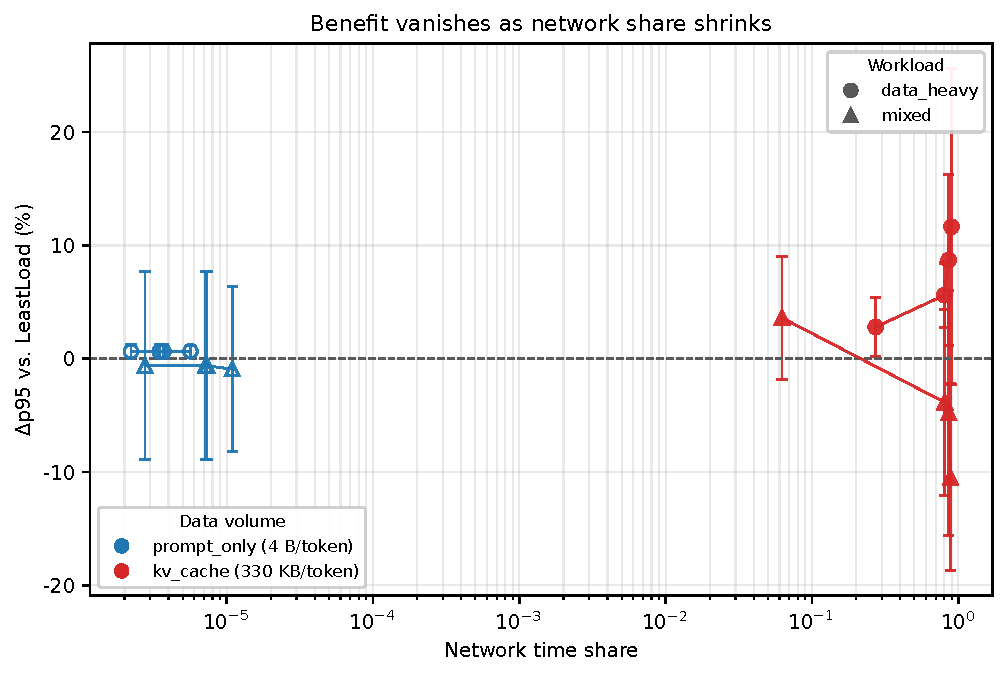
\includegraphics[width=\columnwidth]{fig_benefit_vs_netshare}
\caption{Benefit of the network-aware score against the network-blind baseline as a function of
the fraction of end-to-end time spent moving bytes. Each point is one configuration
(link-scale profile $\times$ workload class) at ten seeds; the two payload regimes are separated
by the vertical gap. Below a network share of a few percent the effect is indistinguishable from
zero.}
\label{fig:netshare}
\end{figure}
The cleanest boundary is the amount of traffic that crosses the network at all. Figure~\ref{fig:netshare} shows it across all four link-scale profiles. Holding
everything else fixed and switching the payload model from KV-cache transfer
(\SI{330}{\kilo\byte}/token) to token-id-only (\SI{4}{\byte}/token) drives the measured network
share from $0.72$--$0.90$ to $0.00$--$0.02$, and the benefit from
$-54.2\%$/$-10.5\%$/$-5.4\%$ (compute-heavy/mixed/low-latency, heterogeneous static network) to
$-1.1\%$/$-0.6\%$/$-0.0\%$. Averaging over four link-scale profiles, the token-id-only regime
yields $\Delta$p95 of $-0.6$ to $+0.7\%$ for every workload --- indistinguishable from zero.
Note this is not a tautology of our network-share gate of \S\ref{sec:policy:adaptive}: the gate
only zeroes \emph{some} decisions (\texttt{w\_gated\_frac} $=0.09$--$0.19$ in the KV regime), and
the residual decisions still have to be scored correctly, which is why the KV regime retains a
$10$--$54\%$ effect rather than disappearing.

\subsection{Alignment: an important explanatory factor for the magnitude}
\label{sec:rq1:alignment}
We now vary \emph{only the pairing} between compute capacity and link bandwidth, holding both
multisets fixed, and re-run the full grid with ten seeds per cell. The result
(Table~\ref{tab:alignment}) is the paper's most robust mechanism finding: when the two rankings
agree ($\rho=+1$), network awareness yields $-3.3\%$ --- statistically distinguishable from zero
but operationally nothing --- while when they maximally disagree ($\rho=-1$) it yields
$-68.2\%$. Group tests over seeds separate the two regimes completely
(Cliff's $\delta=1.00$, Mann--Whitney $p=1.8\times10^{-4}$ for data-heavy/degraded; $\delta\ge
0.94$ and $p\le 4.4\times10^{-4}$ in all four workload$\times$network combinations), and the
pooled trend over the continuous alignment variable is $\rho_s=+0.72$
($p=2.6\times10^{-20}$, $n=120$): the better aligned the configuration, the smaller the benefit. Figure~\ref{fig:alignbars} shows the three alignment configurations side by side.

\begin{table}[t]
\centering
\caption{Alignment sweep (synthetic, 10 seeds, \num{12000} requests/cell; NetworkAware2 vs
LeastLoad). $\rho$ is the Spearman rank correlation between per-worker compute rate and
bandwidth (Eq.~\ref{eq:alignment}), measured on the configuration itself. ``aligned'' is a
control: the network term should add nothing, and does not.}
\label{tab:alignment}
\small
\begin{tabular}{@{}llrrrr@{}}
\toprule
Workload & Network & $\rho$ & $\Delta$p95 (\%) & 95\% CI & $n$ \\
\midrule
\multirow{3}{*}{data-heavy} & \multirow{3}{*}{degraded}
  & $-1.00$ & $-68.2$ & $\pm1.1$ & 10 \\
  & & $+0.50$ & $-30.0$ & $\pm1.3$ & 10 \\
  & & $+1.00$ & $-3.3$ & $\pm2.4$ & 10 \\
\multirow{3}{*}{data-heavy} & \multirow{3}{*}{unstable}
  & $-1.00$ & $-27.0$ & $\pm3.9$ & 10 \\
  & & $+0.50$ & $-26.1$ & $\pm7.3$ & 10 \\
  & & $+1.00$ & $-9.5$ & $\pm2.6$ & 10 \\
\multirow{3}{*}{mixed} & \multirow{3}{*}{degraded}
  & $-1.00$ & $-70.3$ & $\pm1.2$ & 10 \\
  & & $+0.50$ & $-35.4$ & $\pm3.0$ & 10 \\
  & & $+1.00$ & $-22.0$ & $\pm2.8$ & 10 \\
\multirow{3}{*}{mixed} & \multirow{3}{*}{unstable}
  & $-1.00$ & $-26.3$ & $\pm5.2$ & 10 \\
  & & $+0.50$ & $-29.7$ & $\pm7.6$ & 10 \\
  & & $+1.00$ & $-11.7$ & $\pm3.1$ & 10 \\
\bottomrule
\end{tabular}
\end{table}

\subsection{Comparison against standard and mechanism-level baselines}
\label{sec:rq1:baselines}
A reviewer's first question about a result like ours is whether the network-aware family is simply
beating weak baselines. We therefore add four comparison arms chosen so that each answers a
distinct question, all evaluated in the same cells with per-request pairing
(Table~\ref{tab:baselines}).

\textbf{(i) Is the baseline weak?} We compare against power-of-two-choices (P2C), the standard
strong baseline of the load-balancing literature and a fixture of LLM-serving evaluations. In our
setting P2C is \emph{not} a strong baseline: it beats LeastLoad in only $4/8$, $5/8$ and $3/8$
cells on the synthetic, Azure and BurstGPT sources respectively, and on Azure it is worse than
LeastLoad by up to $+17.2\%$. The reason is structural: with three workers in an anti-aligned
configuration, the lower-backlog of two randomly sampled workers is frequently the worker with
the slowest link. Every network-aware arm in this paper beats P2C in at least $6/8$ cells.
Our claim therefore does not rest on weak baselines --- but it also shows that a
\emph{network-blind} two-choice rule is a poor fit for heterogeneous links, which is worth stating
explicitly.

\textbf{(ii) How much does a global view buy?} \textsc{P2CNet} is the same score as
NetworkAware2 but evaluated on two randomly sampled workers instead of all of them. Across the 24
cells of three sources it wins 13 and loses 11 --- a coin flip --- and on the trace batches it is
sometimes substantially better (Azure, mixed/degraded/stale: $-63.3\%$ versus NetworkAware2's
$-40.5\%$). \emph{The network term is what matters; seeing every worker is not.} This has a
practical consequence: a network-aware router can be implemented with two probes per request
rather than $N$.

\textbf{(iii) Is the static bandwidth term redundant?} \textsc{CongestionOnly} is the
Aegis-style reduction of our score to its congestion term alone ($\text{backlog} +
\text{link drain}$), omitting the transfer-time term. It matches NetworkAware2 on the synthetic
source (and beats it in $4/8$ cells there, e.g.\ data-heavy/degraded/fresh: $-74.4\%$ versus
$-68.2\%$), but on both traces it is materially worse, especially once state is stale (Azure,
mixed/degraded/stale: $-27.9\%$ versus $-40.5\%$; data-heavy/degraded/stale: $-31.5\%$ versus
$-41.1\%$). The bandwidth term is therefore not redundant; a congestion-only score is sufficient
only when the links' widths are already known to the router.

\textbf{(iv) Max or sum?} \textsc{Bottleneck} replaces the sum of compute and network time with
their maximum, which is the resource-bottleneck view a max-flow placement takes. On the synthetic
source the sum wins in $8/8$ cells; on both traces the two are indistinguishable ($4/8$ each).
We read this as: at three workers with an anti-aligned configuration, the two resources are
\emph{substitutable} enough that summing is at least as good, and it is simpler.

\begin{table*}[t]
\centering
\caption{Baselines vs.\ the network-blind reference (10 seeds, $\Delta$p95 vs.\ LeastLoad, \%,
negative is better). ``P2C'' = power-of-two-choices on backlog; ``P2CNet'' = two-choice on the
network-aware score; ``Cong.\ only'' = congestion term alone (Aegis-style); ``Bottleneck'' =
$\max(\text{compute},\text{network})$ (Helix-style). ``NA2'' = NetworkAware2.}
\label{tab:baselines}
\small
\setlength{\tabcolsep}{6pt}
\resizebox{\linewidth}{!}{%
\begin{tabular}{@{}llrrrrr@{}}
\toprule
Source & Cell & P2C & P2CNet & Cong.\ only & Bottleneck & NA2 \\
\midrule
Synthetic & d-heavy/degr./fresh & $+5.6$ & $-69.8$ & $\mathbf{-74.4}$ & $-66.4$ & $-68.2$ \\
Synthetic & mixed/unst./stale  & $-14.4$ & $-24.2$ & $-11.5$ & $-6.9$ & $-8.0$ \\
Azure & d-heavy/degr./fresh & $+17.2$ & $-76.2$ & $-76.4$ & $\mathbf{-77.8}$ & $-76.7$ \\
Azure & mixed/degr./stale  & $-6.5$ & $\mathbf{-63.3}$ & $-27.9$ & $-43.5$ & $-40.5$ \\
Azure & d-heavy/unst./stale & $-25.8$ & $-27.9$ & $-0.3$ & $+0.8$ & $-2.0$ \\
BurstGPT & mixed/degr./stale & $-15.9$ & $\mathbf{-50.1}$ & $-30.2$ & $-34.2$ & $-40.8$ \\
BurstGPT & mixed/unst./stale & $-23.3$ & $-20.1$ & $+2.1$ & $+1.2$ & $+7.2$ \\
\midrule
\multicolumn{2}{@{}l}{cells beating LeastLoad (max.\ 8)} & $3$--$5$ & $7$--$8$ & $6$--$8$ & $6$--$8$ & $6$--$8$ \\
\bottomrule
\end{tabular}%
}
\end{table*}

\begin{figure}[t]
\centering
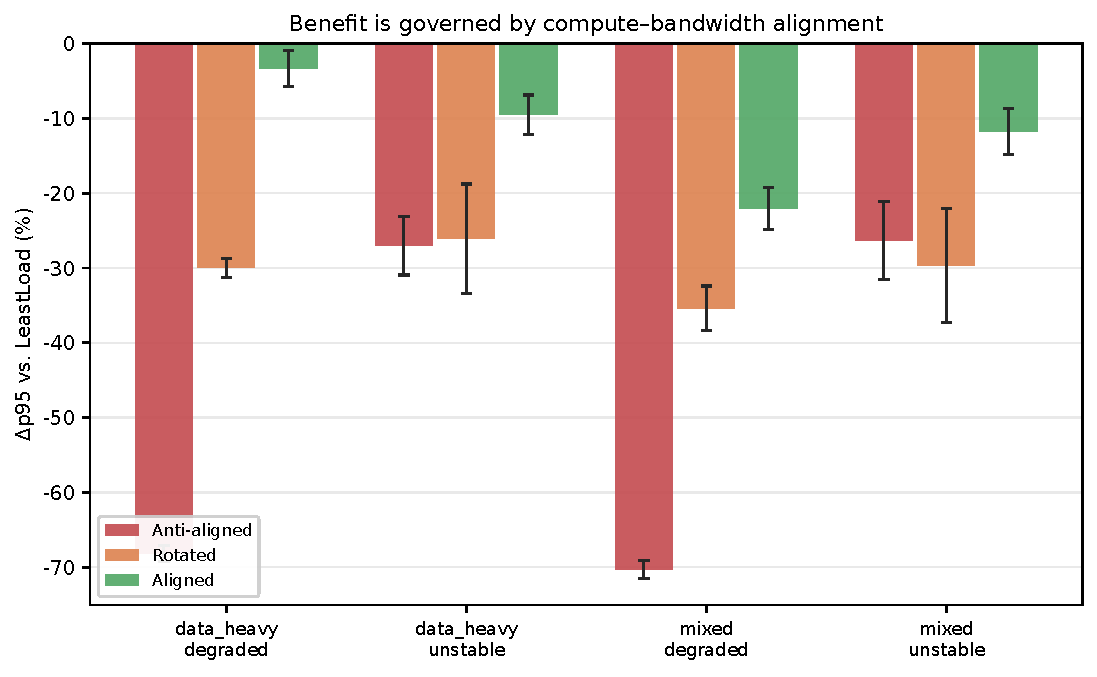
\includegraphics[width=\columnwidth]{fig_alignment_bars}
\caption{Benefit against the network-blind baseline for the three alignment configurations, four
workload$\times$network combinations, ten seeds each. Error bars are $95\%$ confidence intervals
over seeds. The aligned control sits at the origin; the anti-aligned configuration carries the
effect.}
\label{fig:alignbars}
\end{figure}
\begin{figure}[t]
\centering
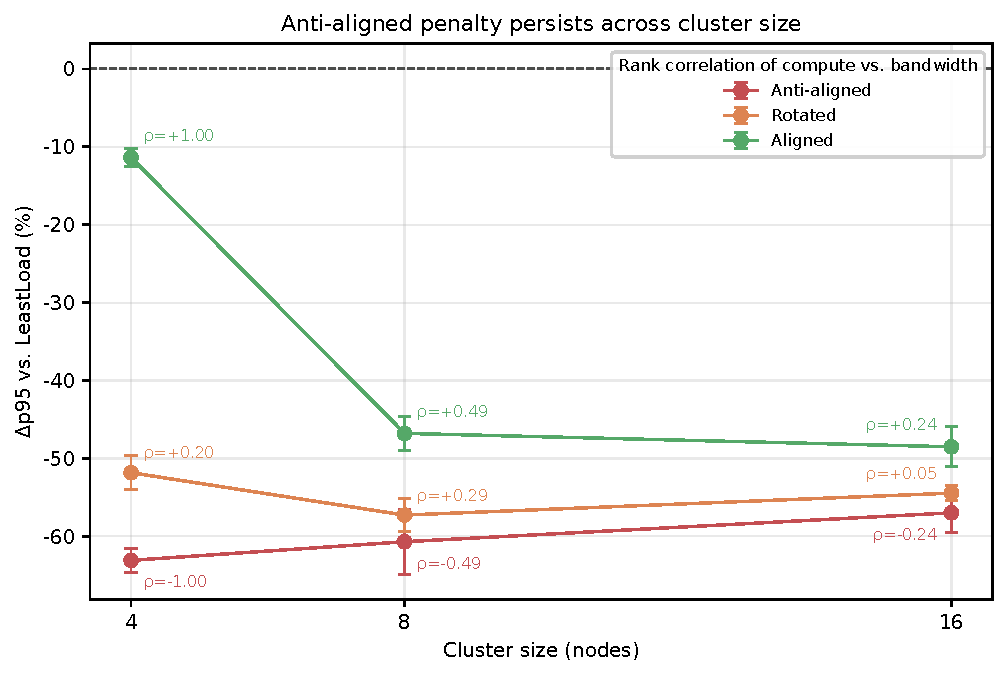
\includegraphics[width=\columnwidth]{fig_alignment_vs_scale}
\caption{The anti-aligned penalty as a function of cluster size, with the rank correlation
$\rho$ annotated at each point. The penalty is flat; what shrinks with size is the attainable
contrast (the $\rho$ values themselves).}
\label{fig:alignscale}
\end{figure}
\subsection{Does the effect survive scale, and is it real?}
Two natural objections follow. First, is the alignment effect an artifact of a three-worker
configuration? We re-run at 4, 8 and 16 workers. The anti-aligned penalty is essentially
\emph{flat} with size: $-63.1\%$, $-60.7\%$, $-57.0\%$ (all $p\le1.7\times10^{-3}$, Cliff
$\delta\ge0.84$). What \emph{does} shrink is the attainable contrast: with a compute ladder of
period four and an $N$-step bandwidth ramp, the extreme correlations become unreachable
($|\rho|$: $1.00$ at $N{=}3,4$; $0.49$ at $N{=}8$; $0.24$ at $N{=}16$). Within each size the
trend is still monotone and significant ($\rho_s=+0.94,+0.82,+0.78$). Reporting
``the effect decays with scale'' would therefore be wrong: the deployed (anti) benefit is
scale-robust, and what decays is our ability to construct a well-aligned \emph{control} at large
$N$ --- a manipulation limitation we disclose rather than a mechanism.

Second, could the benefit simply be LeastLoad ``getting lucky'' with links at larger sizes? We
probe this directly by recording, for every routed request, the bandwidth \emph{rank} of the
worker chosen (rank $1$ = widest link). Under the deployed anti-aligned configuration, LeastLoad
lands at ranks $2.08$, $2.88$, $4.57$, $7.93$ at $N=3,4,8,16$ against random-choice values of
$2.0$, $2.5$, $4.5$, $8.5$ --- i.e.~at or worse than random, never luckier (mean deviation
$0.28$ ranks over the whole range). Under the \emph{aligned} configuration it does land on good
links ($1.44$, $1.61$, $3.37$, $6.59$), and increasingly so with size, which is exactly why the
control benefit grows there. Figure~\ref{fig:alignscale} plots the penalty against cluster size, with the attained $\rho$ annotated at each point. The two configurations therefore differ in what a network-blind
router can achieve, not in whether that router is ``lucky''.

A third objection --- that our results are an artifact of the evaluator's own choices --- we
address in \S\ref{sec:threats}: the SLO definition, the two data-volume regimes, and the fact
that all four engineering coefficients are declared estimates. On load intensity we report a
caveat rather than a curve: the intensity sweep was run with the weaker $v_1$ score, and across
target intensities $0.30$--$0.90$ its effect on p95 ranges from $-15.6\%$ to $+30.8\%$
(mean per intensity level: $-3.0,+6.3,+0.3,-1.9,-2.7\%$, i.e.~no stable sign at all). The
$v_2$ results in this paper are all measured at $\rho=0.6$; extending the \emph{$v_2$} boundary
along the intensity axis is left as future work, and we flag it as the single largest gap in our
coverage.

\section{RQ2: How Fast Does Observed State Expire?}
\label{sec:rq2}

\subsection{Two channels, one grid}
\begin{figure}[t]
\centering
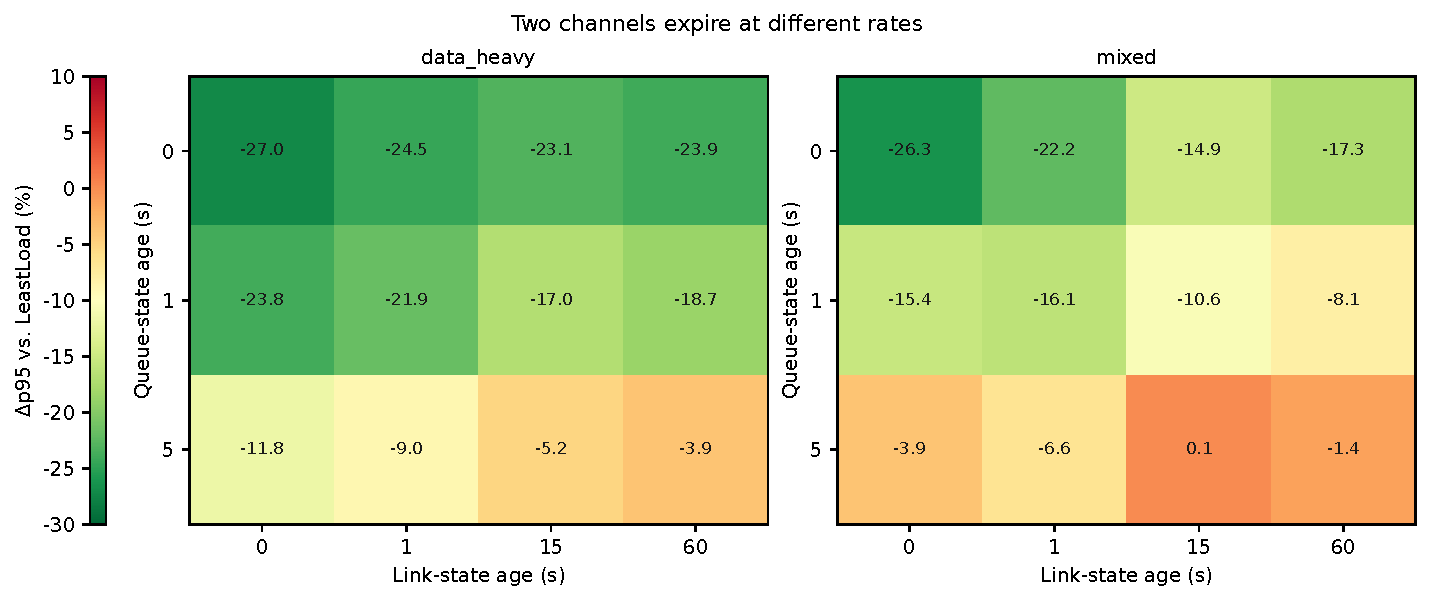
\includegraphics[width=\columnwidth]{fig_staleness_2d}
\caption{Joint staleness grid: benefit of the network-aware score relative to the network-blind
baseline as a function of link-state age (columns) and queue-state age (rows), on the volatile
network. Moving right costs little; moving down is expensive.}
\label{fig:staleness2d}
\end{figure}
We sweep queue age and link age \emph{jointly} (grid $\{0,1,5\}\,\text{s} \times
\{0,1,15,60\}\,\text{s}$, ten seeds, volatile network, since static networks make link age
exactly ineffective). Table~\ref{tab:staleness2d} and Fig.~\ref{fig:staleness2d} give the result. Two readings matter.

\begin{table}[t]
\centering
\caption{Joint staleness grid (synthetic, 10 seeds, NetworkAware2 vs LeastLoad, $\Delta$p95 in
\%). Rows: queue age; columns: link age. Reading down a column isolates link age; reading across
a row isolates queue age.}
\label{tab:staleness2d}
\small
\begin{tabular}{@{}lrrrr@{}}
\toprule
\multicolumn{1}{c}{} & \multicolumn{4}{c}{link age} \\
\cmidrule(lr){2-5}
queue age & \SI{0}{\second} & \SI{1}{\second} & \SI{15}{\second} & \SI{60}{\second} \\
\midrule
\multicolumn{5}{@{}l}{\emph{data-heavy}}\\
\SI{0}{\second}  & $-27$ & $-25$ & $-23$ & $-24$ \\
\SI{1}{\second}  & $-24$ & $-22$ & $-17$ & $-19$ \\
\SI{5}{\second}  & $-12$ & $-9$  & $-5$  & $-4$  \\
\midrule
\multicolumn{5}{@{}l}{\emph{mixed}}\\
\SI{0}{\second}  & $-26$ & $-22$ & $-15$ & $-17$ \\
\SI{1}{\second}  & $-15$ & $-16$ & $-11$ & $-8$  \\
\SI{5}{\second}  & $-4$  & $-7$  & $0$   & $-1$  \\
\bottomrule
\end{tabular}
\end{table}

First, \textbf{link state barely expires}. Holding the queue fresh, moving the link snapshot from
\SI{0}{\second} to \SI{60}{\second} leaves $89\%$ of the benefit for data-heavy traffic
($-27\%\rightarrow-24\%$) and $65\%$ for mixed ($-26\%\rightarrow-17\%$). This is not an
artifact of the static control: these cells are on the volatile network.

Second, \textbf{queue state expires fast, and the two compose}. Holding the link fresh, going
from \SI{0}{\second} to \SI{5}{\second} of queue age costs $56\%$ of the benefit for mixed
($-26\%\rightarrow-4\%$) and $56\%$ for data-heavy ($-27\%\rightarrow-12\%$). The two impairments
compound: with both channels old ($5\,\text{s}/60\,\text{s}$) the benefit is $-4\%$ (data-heavy)
and $-1\%$ (mixed), i.e.~smaller than either impairment alone would predict.
Comparing the channels at equal age is not meaningful: \emph{five seconds} of queue age destroys
$56$--$85\%$ of the benefit, whereas \emph{sixty seconds} of link age destroys only
$11$--$35\%$. Fitting a single exponential to each channel is not something two points per
channel supports, but the ordering is unambiguous and large: the queue channel's effective time
constant is roughly an order of magnitude (or more) smaller than the link channel's.

\paragraph{Why.} The two observables differ in what they are made of. A link's \emph{bandwidth}
is a slowly varying physical property, so even an old link snapshot still ranks workers almost
correctly on the structural part; only the congestion part is perishable. A compute queue has no
such structural component: it is entirely a statement about ``right now'', and it becomes wrong
at the rate the system's load changes. This observation is what makes the published
``telemetry delayed by \SI{60}{\second} does not matter'' finding \cite{aegis} both reproducible
and incomplete: the quantity swept was the slow-expiring channel.

\subsection{Latency and averaging are different distortions}
Real monitoring usually reports a \emph{time average} rather than an instantaneous value
(\texttt{avg\_over\_time} over the scrape interval), and a smoothing window is a different defect
from a lag: a lag makes the router react late, whereas averaging hides the very spike the router
is currently inside. We sweep the window independently of the lag (lag $=0$), for each channel.

Averaging inflates \emph{absolute} latency substantially and roughly equally for both policies:
a \SI{30}{\second} queue window moves p95 from \SI{46.2}{\second} to \SI{65.2}{\second} for the
network-aware policy and from \SI{139.6}{\second} to \SI{211.1}{\second} for the network-blind
baseline ($+41\%$ and $+51\%$; mixed/degraded: $+44\%$ and $+52\%$; mixed/unstable: $+46\%$ and
$+35\%$). The \emph{relative} advantage, however, moves much less: on the static network it is
essentially unchanged ($-67.0\%\rightarrow-69.1\%$ for data-heavy, $-71.7\%\rightarrow-69.1\%$
for mixed), and on the volatile network it erodes only moderately
($-20.4\%\rightarrow-14.4\%$ for mixed). Contrast this with the same amount of pure lag, which
at \SI{5}{\second} on the queue channel collapses the benefit to $-4\%$. In other words:
\textbf{for this system, being shown a smoothed average is far less damaging than being shown a
stale value}, which inverts the intuition that ``any loss of freshness is equally bad''. We
report the window channel separately for exactly this reason, and we note that the metric a real
monitoring stack reports---window length, scrape interval, and export delay---determines which of
the two distortions dominates.

\section{Conditional Use of Network State}
\label{sec:discount}

Given \S\ref{sec:rq2}, a natural next step is to discount the network term as its inputs age. We
built four such rules (Eqs.~\ref{eq:hard}--\ref{eq:channel}) and evaluated them in the same cells
as the two extremes (full trust $=$ NetworkAware2; no trust $=$ LeastLoad), ten seeds,
\num{12000} requests per cell, on all three workload sources. The comparison is paired
per-request within a cell, so it measures the rules rather than the configurations.

\subsection{What the first attempt got wrong (a falsified design)}
Our first design discounted \emph{within} the link term, on the hypothesis that a stale link
snapshot retains its structural content (``which link is wide'') while losing its dynamic content
(``who is congesting it now''): it kept the transfer term at full weight and decayed only the
congestion term. The hypothesis is mechanistically appealing and, on this evidence, wrong.
Table~\ref{tab:discount} shows what happened under a \SI{60}{\second}-old link snapshot: on the
Azure trace the term-split rule retains only $-40.2\%$ of the $-76.7\%$ available, whereas
applying a single factor to the whole network term retains $-76.2\%$. On the synthetic source it
is worse still ($+5.5\%$, i.e.~the benefit is destroyed entirely). The mechanism is the mirror
image of an earlier failure we made: muting the congestion penalty makes \emph{fat link, slow
compute} workers attractive again, and traffic piles onto exactly the worker the link term was
supposed to protect. \textbf{Discounting must be applied at the level of the information source
(the channel), not at the level of an individual score term.}

\begin{table*}[t]
\centering
\caption{Four discounting rules against the two extremes, under a \SI{60}{\second}-old link
snapshot with a fresh queue (all values are $\Delta$p95 vs.\ LeastLoad, \%; negative is better).
``per-channel'' is Eq.~\ref{eq:channel}, ``term-split'' is the falsified design
Eq.~\ref{eq:split}; ``uniform'' and ``hard'' are Eqs.~\ref{eq:linear} and~\ref{eq:hard}.
Values in parentheses are medians, given only where the trace batches' per-seed spread is large.}
\label{tab:discount}
\small
\setlength{\tabcolsep}{5pt}
\resizebox{\linewidth}{!}{%
\begin{tabular}{@{}llrrrrr@{}}
\toprule
Source & Cell & full trust & per-channel & term-split & uniform & hard \\
\midrule
Synthetic & d-heavy / degraded & $-68.2$ & $-61.2$ & $+5.5$ & $0.0$ & $0.0$ \\
Synthetic & mixed / degraded   & $-70.3$ & $-66.2$ & $-16.6$ & $0.0$ & $0.0$ \\
Azure     & d-heavy / degraded & $-76.7$ & $\mathbf{-76.2}$ & $-40.2$ & $+0.1$ & $+0.1$ \\
Azure     & mixed / degraded   & $-76.8$ & $\mathbf{-74.4}$ & $-31.1$ & $+0.7$ & $+0.5$ \\
BurstGPT  & mixed / degraded   & $-60.1$ & $-58.8$ & $-28.7$ & $-20.7$ & $-10.6$ \\
BurstGPT  & mixed / unstable, $5/60$\,s & $+32.5$ {\scriptsize$(+23.4)$} & $\mathbf{+3.0}$ {\scriptsize$(-0.1)$} & $+1.7$ & $-3.3$ & $+2.5$ \\
\bottomrule
\end{tabular}%
}
\end{table*}

\subsection{What the corrected rule buys, and what it does not}
\begin{figure}[t]
\centering
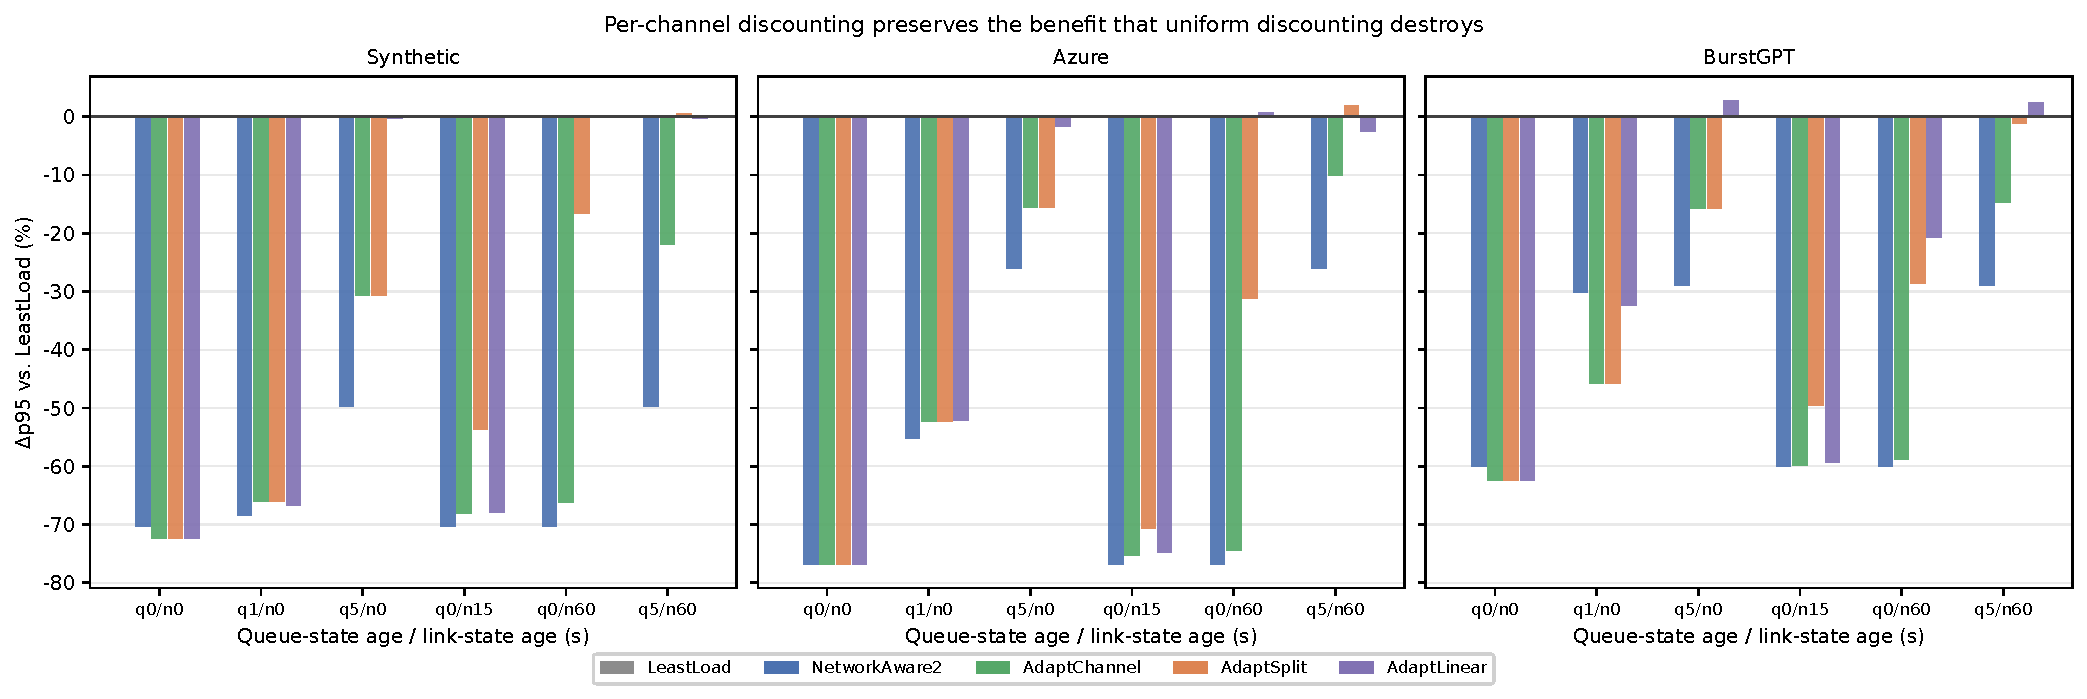
\includegraphics[width=\columnwidth]{fig_discount_rules}
\caption{The four discounting rules against both extremes, on the three workload sources
(mixed workload, heterogeneous static network). Per-channel discounting tracks full trust where
the link snapshot is old, while uniform and threshold discounting collapse to the network-blind
baseline.}
\label{fig:discount}
\end{figure}
The per-channel rule keeps $90$--$99\%$ of the available benefit under a \SI{60}{\second}-old
link snapshot on all three sources (Azure: $-76.7\%\rightarrow-76.2\%$; synthetic:
$-68.2\%\rightarrow-61.2\%$; BurstGPT: $-60.1\%\rightarrow-58.8\%$), where the uniform and hard
alternatives destroy \emph{all} of it. Figure~\ref{fig:discount} shows all four rules against both extremes on all three workload sources. In the language of \S\ref{sec:rq2}, this is expected: the
link channel's value barely decays, so \emph{any} discount applied to it mostly subtracts value.

The rule is not free, and we report where it loses (Table~\ref{tab:verdict}). It is a net loss in
the majority of conditions on the Azure source, and it never dominates the two extremes; what it
buys is the absence of a specific failure mode. That failure mode is visible in the last row of
Table~\ref{tab:discount}: on the burstiest source, with both channels stale, full trust is
\emph{harmful} (median $+23.4\%$, i.e.~the network-aware policy is worse than the policy that
ignores the network in the majority of seeds), and the per-channel rule removes that harm
(median $-0.1\%$). We emphasize that we found this only after replacing the mean of per-seed
relative differences with its median: the mean at that cell is $+32.5\%$ while the median is
$+23.4\%$ (both harmful, so the conclusion is robust \emph{here}), but at a neighbouring cell
(data-heavy/unstable, $5/0$) the mean is $+27.8\%$ while the median is $-0.5$ --- a
single-seed artifact that a mean-only table would have promoted to a finding.

\begin{table}[t]
\centering
\caption{Verdict counts over 24 conditions per source (6 staleness configurations $\times$ 2
workloads $\times$ 2 network conditions). ``Better than both'' counts conditions where the rule
beats \emph{both} full trust and no trust. No rule dominates.}
\label{tab:verdict}
\footnotesize
\setlength{\tabcolsep}{4pt}
\begin{tabular}{@{}lrrrrr@{}}
\toprule
Source & Rule & beats both & loses both & beats full & loses full \\
\midrule
\multirow{4}{*}{Synthetic} & per-channel & 5 & 1 & 5 & 18 \\
                           & term-split  & 4 & 3 & 4 & 19 \\
                           & uniform     & 5 & 5 & 5 & 18 \\
                           & hard        & 5 & 1 & 5 & 17 \\
\midrule
\multirow{4}{*}{Azure}     & per-channel & 1 & 4 & 1 & 22 \\
                           & term-split  & 1 & 5 & 1 & 22 \\
                           & uniform     & 2 & 4 & 4 & 19 \\
                           & hard        & 4 & 8 & 7 & 15 \\
\midrule
\multirow{4}{*}{BurstGPT}  & per-channel & 8 & 2 & 10 & 13 \\
                           & term-split  & 6 & 2 & 8 & 15 \\
                           & uniform     & 10 & 4 & 10 & 13 \\
                           & hard        & 7 & 3 & 8 & 14 \\
\bottomrule
\end{tabular}
\end{table}

\subsection{When is discounting actually needed?}
The robust way to ask this is not ``how large is the effect'' but ``in how many independent seeds
does full trust lose to the network-blind baseline''. Table~\ref{tab:seedcount} answers it, and
the answer is sharply localized. With a fresh queue, full trust wins in $9$--$10$ of $10$ seeds
even when the link snapshot is \SI{60}{\second} old --- discounting there is pure loss. On the
\emph{volatile} network with a \SI{5}{\second}-old \emph{queue}, full trust loses in 4--6 of 10
seeds on all three sources. That single cell is where discounting has a job to do, and it is
exactly the regime that the two-channel expiry model of \S\ref{sec:rq2} predicts.

\begin{table}[t]
\centering
\caption{Seeds (of 10) in which full trust beats the network-blind baseline. The only regime
where full trust is unreliable is a stale queue on a volatile network.}
\label{tab:seedcount}
\footnotesize
\setlength{\tabcolsep}{3pt}
\begin{tabular}{@{}llrrr@{}}
\toprule
Queue / link age & Source & mixed / deg. & mixed / unst. & d-heavy / unst. \\
\midrule
$0/60$\,s & Synthetic & 10 & 10 & 10 \\
$0/60$\,s & Azure     & 10 & 9  & 10 \\
$0/60$\,s & BurstGPT  & 10 & 9  & 6  \\
\midrule
$5/0$\,s  & Synthetic & 10 & 6  & 10 \\
$5/0$\,s  & Azure     & 10 & 4  & 4  \\
$5/0$\,s  & BurstGPT  & 8  & 7  & 5  \\
\bottomrule
\end{tabular}
\end{table}

\subsection{Parameter sensitivity}
\begin{figure}[t]
\centering
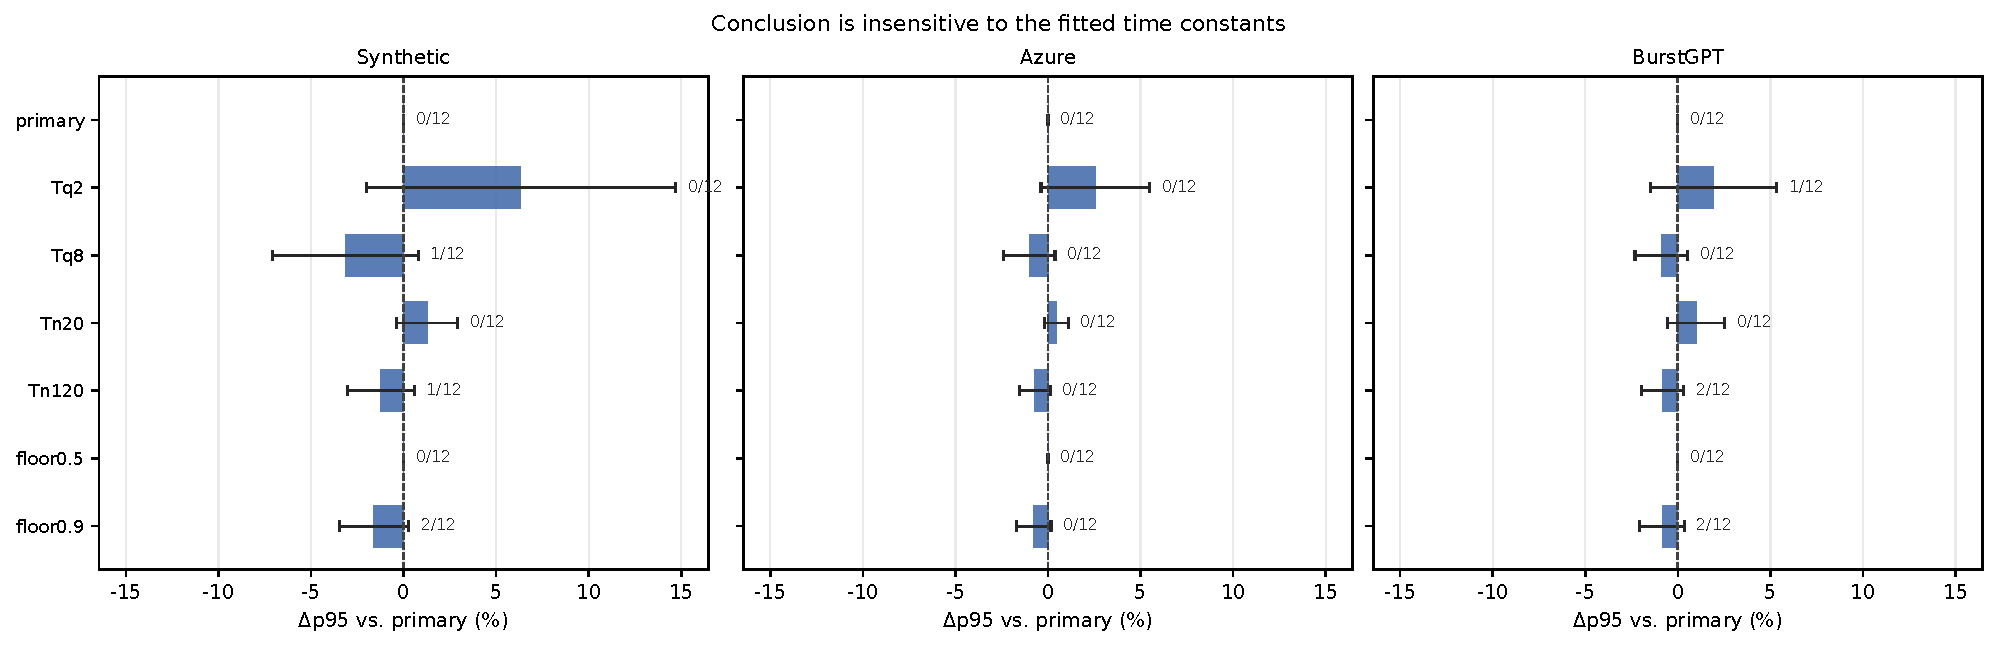
\includegraphics[width=\columnwidth]{fig_ablation}
\caption{One-factor-at-a-time ablation of the per-channel rule on all three sources. Bars show
the mean change in p95 relative to the unmodified rule with $95\%$ confidence intervals; the
annotation on each bar counts conditions where the sign of the conclusion changes.}
\label{fig:ablation}
\end{figure}
The rule of Eq.~\ref{eq:channel} has exactly three numbers, all read off the measured curves of
\S\ref{sec:rq2} rather than tuned. We ablate each by a factor of two, one at a time, on all three
sources (Table~\ref{tab:ablation}). Moving the link-side time constant between \SI{20}{\second}
and \SI{120}{\second} changes p95 by $-1.2$ to $+1.3\%$; moving the weight floor between $0.5$
and $0.9$ changes it by $-1.6$ to $0.0\%$; moving the queue-side constant between \SI{2}{} and
\SI{8}{\second} changes it by $-3.2$ to $+6.3\%$, with the confidence interval spanning zero. The
\emph{direction} of the conclusion (does the rule beat full trust?) flips in at most 2 of 12
conditions on any source, and in 0 of 12 on Azure. Figure~\ref{fig:ablation} summarizes the ablation across sources. The parameters are therefore not load-bearing individually
individually, which is what one wants from constants that are supposed to be read off data.

\begin{table}[t]
\centering
\caption{One-factor-at-a-time ablation of the per-channel rule (mean $\Delta$p95 vs.\ the
unmodified rule, with 95\% CI over 12 conditions; ``flips'' counts conditions where the
sign of ``rule vs.\ full trust'' changes).}
\label{tab:ablation}
\footnotesize
\setlength{\tabcolsep}{4pt}
\begin{tabular}{@{}lrrrr@{}}
\toprule
Variant & Synthetic & Azure & BurstGPT & flips (max) \\
\midrule
$\tau_q: 4\rightarrow2$\,s & $+6.3\pm8.4$ & $+2.6\pm2.9$ & $+1.9\pm3.4$ & 1/12 \\
$\tau_q: 4\rightarrow8$\,s & $-3.2\pm3.9$ & $-1.0\pm1.4$ & $-0.9\pm1.4$ & 1/12 \\
$\tau_n: 60\rightarrow20$\,s & $+1.3\pm1.7$ & $+0.4\pm0.6$ & $+1.0\pm1.5$ & 0/12 \\
$\tau_n: 60\rightarrow120$\,s & $-1.2\pm1.8$ & $-0.7\pm0.8$ & $-0.8\pm1.1$ & 2/12 \\
floor: $0.7\rightarrow0.5$ & $0.0\pm0.0$ & $0.0\pm0.0$ & $0.0\pm0.0$ & 0/12 \\
floor: $0.7\rightarrow0.9$ & $-1.6\pm1.9$ & $-0.8\pm0.9$ & $-0.9\pm1.2$ & 2/12 \\
\bottomrule
\end{tabular}
\end{table}

\subsection{What we could not explain}
The natural next question is \emph{what property of the load determines whether discounting
pays?} We pre-registered two hypotheses and both failed. \emph{H1:} harm grows with arrival
burstiness. Ordering the three sources by per-second arrival-count variability gives Azure
($0.23$--$0.30$) $<$ synthetic ($0.60$--$0.65$) $<$ BurstGPT ($1.30$--$2.11$), but the fraction
of the benefit destroyed by a \SI{5}{\second} queue age is largest on Azure, not on BurstGPT ---
not monotone.\footnote{We also measured rate \emph{persistence} (lag-1 autocorrelation of
per-second counts, and the mean relative change of the 5-second windowed rate), on the hypothesis
that a transient rate spike is harmless because it averages out while a sustained one is not.
Synthetic has the \emph{highest} autocorrelation ($0.73$--$0.85$) and the \emph{lowest} harm,
which refutes that hypothesis as well.} We therefore state the boundary as measured --- a stale
queue on a volatile network, on all three sources --- and leave the mechanism open, noting that
a scale-matching explanation (staleness matters when the observation window is comparable to the
queue's own drain time) is consistent with our data but is not something we tested. A related
observation from the literature, that performance collapses when a controller's timescale fails
to match the machine's \cite{dlfp}, suggests a concrete next experiment.

\section{Real-Cluster Measurements}
\label{sec:real}

Simulation gives us control but assumes away the cost of knowing. We therefore ran the same
routing logic on real containers (\S\ref{sec:setup:real}): a single-node \texttt{k3s} cluster with
three worker pods, application-level link shaping, and a client outside the cluster. We report
three things the simulator cannot see, then the reproducibility of the comparison itself.

\subsection{The benefit needs network share, and tolerates little staleness}
At an offered load corresponding to $\rho_{\text{cpu}}=0.50$ and a \SI{38.9}{\mega\byte} payload
(measured network share $0.65$), the network-aware policy beats the network-blind one in four of
four grid cells, by $21$--$45\%$ on p95. At a \SI{0.6}{\mega\byte} payload (network share
$0.05$) the same comparison is $-1.6\%$, $+68.7\%$, $+23.1\%$, $-16.3\%$ --- i.e.~no effect or
harm. This is the same on/off behavior as \S\ref{sec:rq1}, on real kernel networking rather than
a model. Injecting a \SI{3}{\second} state lag reduces the benefit from $-45.2\%$ to $-21.4\%$ at
the moderate load and from $-37.5\%$ to $-27.9\%$ at the higher one, consistent with the
direction found in simulation.

\subsection{Reading state is not free, and gets slower exactly when it matters}
The simulator assumes an observation is instantaneous. On the cluster, fetching a worker's state
costs \SIrange{56}{876}{\milli\second} against \SI{12}{\micro\second} for an in-cluster network
round trip --- a factor of \numrange{50}{900}. More importantly, the cost is not constant: it
grows with system load, because the state endpoint competes for the same CPU quota as the work it
describes. This is a \emph{feedback loop} that simulation omits by construction: the busier the
system, the staler the observation, precisely when freshness matters most.

We also measured the floor that polling imposes. With a \SI{15}{\second} polling period, the
actual age of the state the scheduler acts on was \SI{6.4}{\second} on average and
\SI{14.8}{\second} worst-case --- that is, roughly half a period to a full period, on top of any
export delay. A scheduler cannot be fresher than its polling loop, so ``zero lag'' is not
achievable in practice even when no network delay exists.

Two operational failure modes surfaced. First, the latency impact of stale state is
\emph{threshold-like}, not proportional: pulls taking \SI{64}{\milli\second} to
\SI{755}{\milli\second} left p95 essentially unchanged, whereas pulls taking
\SI{3.6}{\second} to \SI{6.4}{\second} made p95 \numrange{2}{3.6}$\times$ worse. In our setting
the knee sits between \SI{1}{\second} and \SI{5}{\second}. Second, when a state pull times out
(>\SI{2}{\second}), our client substitutes a conservative ``everything is busy'' value, which
makes the scheduler effectively blind; this occurred twice in a long run and is a failure mode
worth designing for explicitly rather than discovering in production.

\subsection{How much can a single-node cluster claim?}
\begin{figure}[t]
\centering
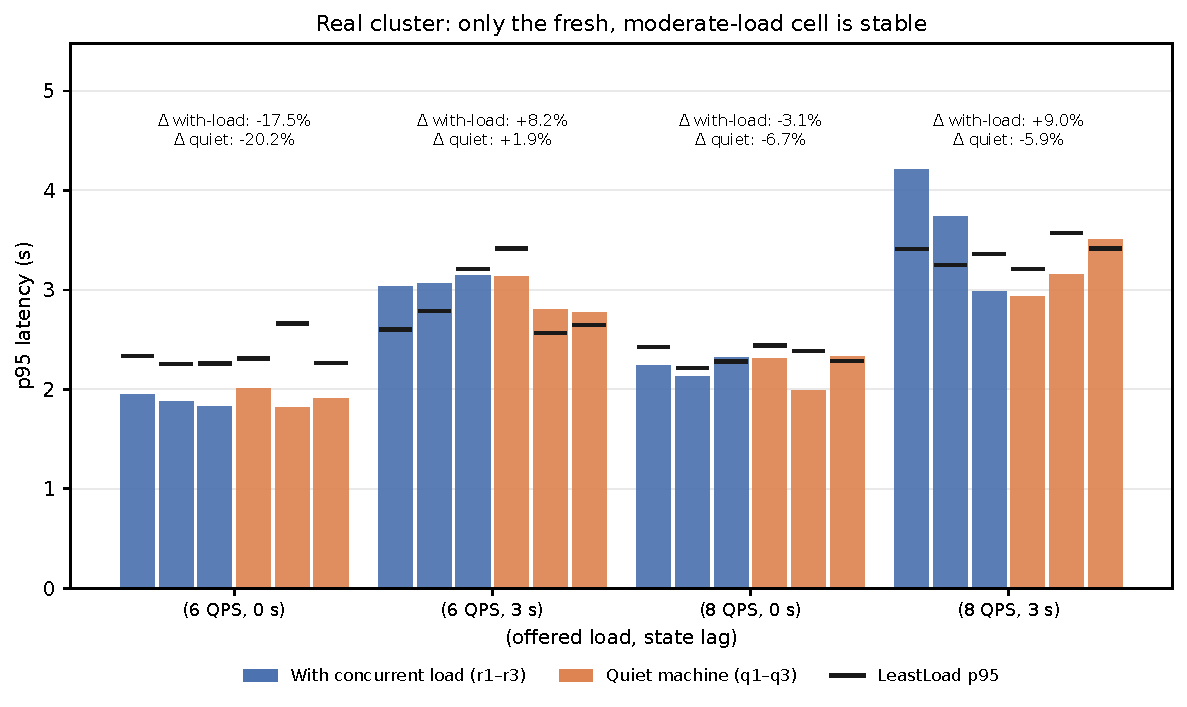
\includegraphics[width=\columnwidth]{fig_real_cluster}
\caption{Real cluster, six independent repeats per cell. Bars are the network-aware policy's p95
under three runs with a concurrent job on the host and three on an idle machine; short horizontal
marks are the network-blind baseline for the same run. Only the fresh, moderate-load cell has a
stable direction across all six.}
\label{fig:real}
\end{figure}
Because the earlier grid ran each cell once, we repeated a focused grid (two offered loads
$\times$ two staleness levels $\times$ the payload with $0.65$ network share) six times, three of
them while a simulation also ran on the same host and three on an otherwise idle machine.

\begin{table}[t]
\centering
\caption{Real cluster, six independent repeats of each cell ($\Delta$p95 of the network-aware
policy vs.\ the network-blind one; negative is better). Only the fresh, moderate-load cell has a
stable direction.}
\label{tab:realrepeats}
\footnotesize
\setlength{\tabcolsep}{4pt}
\begin{tabular}{@{}llrrrrrrr@{}}
\toprule
Load & State & \multicolumn{3}{c}{with a concurrent job} & \multicolumn{3}{c}{idle machine} \\
\cmidrule(lr){3-5}\cmidrule(lr){6-8}
(qps) & lag & 1 & 2 & 3 & 1 & 2 & 3 \\
\midrule
6 & 0\,s & $-16.5$ & $-16.8$ & $-19.2$ & $-13.1$ & $-31.7$ & $-15.6$ \\
6 & 3\,s & $+16.6$ & $+9.9$  & $-1.8$  & $-8.2$  & $+9.4$  & $+4.6$  \\
8 & 0\,s & $-7.5$  & $-3.8$  & $+1.9$  & $-5.4$  & $-16.8$ & $+2.0$  \\
8 & 3\,s & $+23.4$ & $+15.0$ & $-11.4$ & $-8.6$  & $-11.8$ & $+2.7$  \\
\bottomrule
\end{tabular}
\end{table}

Figure~\ref{fig:real} shows the six repeats. Three conclusions follow, one of which is a retraction of our own earlier observation.
(i) The only direction that is stable across all six repeats is the fresh, moderate-load cell:
the network-aware policy is better, six times out of six, by $13$--$32\%$.
(ii) At the higher load, and in every stale cell, the sign is not stable; the honest statement is
that a single-node cluster cannot resolve it.
(iii) We initially observed, in the three concurrent runs, that the network-aware policy's tail
latency became far more variable across repeats than the baseline's ($\pm17\%$ vs.\ $\pm2.4\%$ at
qps\,8 with \SI{3}{\second} staleness) and considered reporting it as a finding. The idle-machine
repeats do not reproduce it (baseline $10.8\%$ vs.\ policy $18.0\%$; at qps\,6 the ordering even
reverses). We therefore withdraw the claim: it was an artifact of three runs, and it is exactly
the kind of conclusion that single-run, mean-only tables produce.

The most useful number here is not any of the deltas but their spread: repeat-to-repeat
dispersion is \SIrange{10}{30}{\percent} on an \emph{idle} machine, so a single run of this
testbed supports direction and nothing more. We report this because it retroactively bounds the
confidence of our own earlier single-run grid (\S\ref{sec:real}, first paragraph), whose larger
deltas should be read as an optimistic estimate rather than a magnitude.

\subsection{Cloud disaggregation: same-cloud baseline and cross-cloud feasibility}
\label{sec:real:cloud}

The container experiment above validates the direction of the simulation mechanism, but it does
not measure a real LLM service or a cross-cloud KV path. We therefore ran a separate, tightly
scoped measurement with Qwen2.5-1.5B-Instruct on A10 instances. This experiment is a feasibility
and deployment anchor, not a population-level statistical study: B2 used four paired service
rounds, while C used two cloud directions. Requests inside a round or direction are repeated
observations, not independent experiments.

Table~\ref{tab:cloudcost} summarizes the anchor. In the same-cloud baseline, splitting prefill
and decode increased median time to first token (TTFT) by $207.3\%$ in serial execution and
$97.1\%$ at concurrency four, while the average token interval changed by only $+1.3\%$ and
$-1.5\%$. Total median latency increased by $16.0\%$ and $9.8\%$. The KV ledger was
independently consistent: each split round transferred $100$ KV objects and about $4.294$ GB,
with zero transfer failures and zero local prompt recomputation.

The cross-cloud feasibility run completed both directions and all $200$ formal requests, with
zero failures and exactly $64$ generated tokens per request. Relative to the same-cloud split
baseline, serial TTFT increased by $1872\%$ for Alibaba-to-Tencent and $1720\%$ for
Tencent-to-Alibaba; at concurrency four the corresponding descriptive changes were $5289\%$
and $5211\%$. These values are not universal cloud penalties: the two directions used different
client locations, asymmetric paths, tunnel conditions, and non-identical GPU software
environments. They show that, in this deployment, the dominant extra cost appears before the
first generated token, whereas the decode stream is comparatively stable.

\begin{table}[t]
\centering
\caption{Real-LLM deployment anchor. Values are medians unless a range is shown. B2 is a
descriptive baseline over four paired rounds; C is a descriptive feasibility measurement over two
directions. The C values are not inferential estimates.}
\label{tab:cloudcost}
\scriptsize
\setlength{\tabcolsep}{3pt}
\resizebox{\columnwidth}{!}{%
\begin{tabular}{@{}llrrrrl@{}}
\toprule
Shape & Load & TTFT p50 & TTFT p95 & Token gap & Total p50 & Evidence unit \\
\midrule
Base & serial & 0.068 & 0.122 & 0.0141 & 0.953 & B2, 4 rounds \\
Same-cloud split & serial & 0.211 & 0.321 & 0.0142 & 1.111 & B2, 4 rounds \\
Alibaba $\rightarrow$ Tencent & serial & 4.16 & 7.10 & 0.0177 & 5.26 & C, D1 \\
Tencent $\rightarrow$ Alibaba & serial & 3.84 & 6.39 & 0.0144 & 4.78 & C, D2 \\
\midrule
Base & concurrency 4 & 0.144 & 0.309 & 0.0164 & 1.204 & B2, 4 rounds \\
Same-cloud split & concurrency 4 & 0.280 & 0.648 & 0.0162 & 1.301 & B2, 4 rounds \\
Alibaba $\rightarrow$ Tencent & concurrency 4 & 15.09 & 18.46 & 0.0191 & 16.25 & C, D1 \\
Tencent $\rightarrow$ Alibaba & concurrency 4 & 14.87 & 21.30 & 0.0171 & 15.95 & C, D2 \\
\midrule
\multicolumn{7}{l}{KV ledger: $28{,}798.9$ bytes/token; $100$ transfers/round; failures $=0$; local recomputation $=0$.}\\
\bottomrule
\end{tabular}%
}
\end{table}

Figure~\ref{fig:cloudttft}(a) places the four deployment forms on the same descriptive scale.
Figure~\ref{fig:cloudttft}(b) shows the five C-stage prompt-length groups as a descriptive
background. The dashed lines are anchored engineering references based on measured bandwidth,
not fitted regressions; D-mini was planned but not executed. Thus the figure illustrates the
transport-dominated regime without claiming a general linear scaling law.

\begin{figure}[t]
\centering
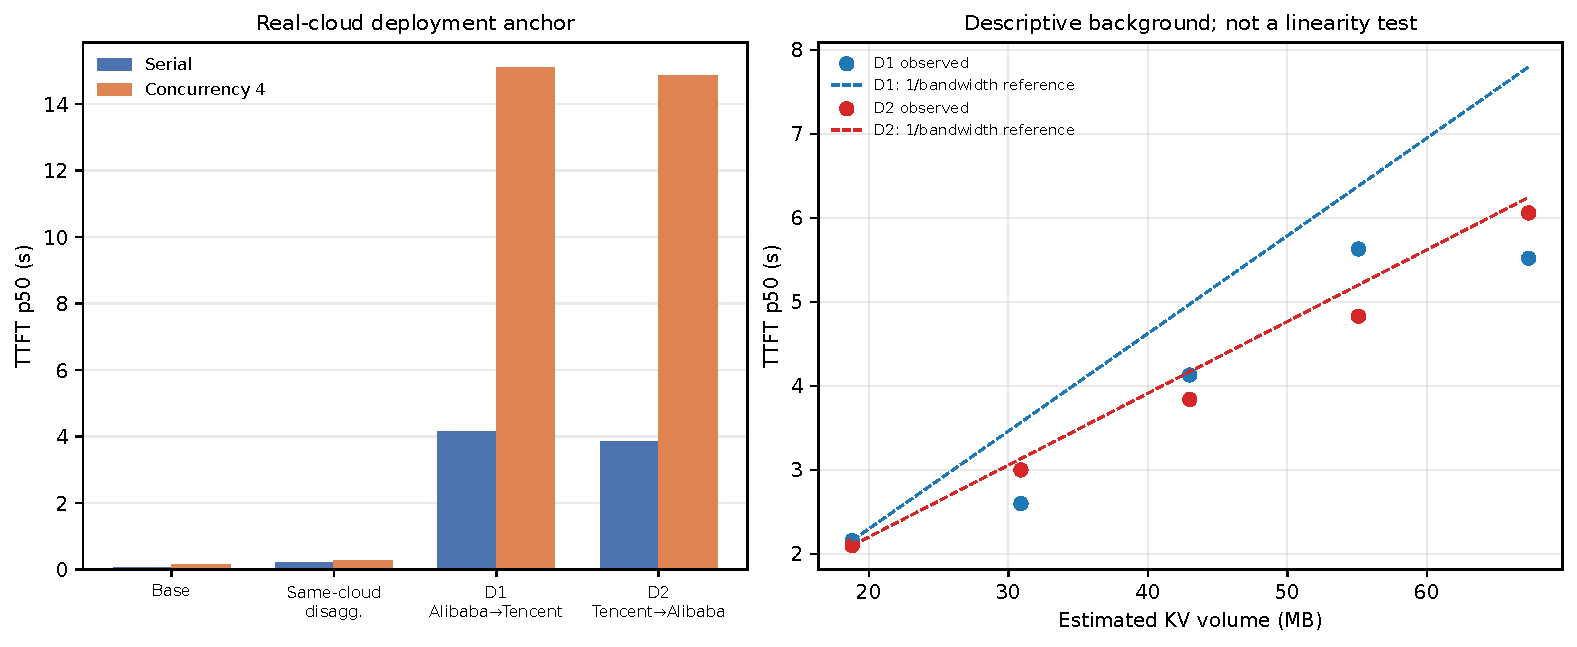
\includegraphics[width=\columnwidth]{fig_cloudttft}
\caption{Real-cloud deployment anchor. (a) Median TTFT for same-cloud and cross-cloud
configurations under serial and four-way concurrency. (b) C-stage TTFT against estimated KV
volume for five fixed prompt groups. Dashed lines are anchored $1/\mathrm{bandwidth}$ engineering
references; this panel is a \emph{descriptive background}, not a linearity test. D-mini was planned
but not executed.}
\label{fig:cloudttft}
\end{figure}

\section{Threats to Validity}
\label{sec:threats}

\paragraph{Serving model.} Each worker's slots advance at full speed independently, so total
throughput is the linear sum of per-slot rates. Real GPU concurrency does not work that way: when
we measured a real \num{4}-way parallel serving process, per-request service time rose from
\SI{83}{\milli\second} idle to \SI{162}{\milli\second} at sustained saturation ($1.95\times$).
In the saturated region our simulator therefore \emph{overestimates} throughput by roughly a
factor of two, which inflates the achievable throughput against a fixed SLO; the p95 comparisons
between policies are less affected because all policies share the error, but this is an
assumption, not a measurement.

\paragraph{Network model.} Transfers are serialized on a per-worker pipe and the transfer
\emph{rate} does not degrade as more requests share it; multiple concurrent transfers are FIFO
rather than processor-shared, and inter-worker links are independent (no shared uplink, no
incast, no fabric-level queueing, no congestion control). This \emph{underestimates} network cost
at high load, i.e.~makes our reported benefits conservative. The real-cluster testbed shapes
bandwidth in the application layer rather than with \texttt{tc}; the kernel path (socket buffers,
loopback of a container network) is real, the shaping is not.

\paragraph{Cluster evidence.} Our real deployment is a \emph{single} node: containers with CPU
quotas, no GPUs, no RDMA, no multi-host fabric. It can establish direction and can measure the
cost of reading state; it cannot establish production magnitudes. We quantify this rather than
assert it: repeat-to-repeat dispersion on an idle machine is \SIrange{10}{30}{\percent}
(\S\ref{sec:real}), so every real-cluster delta in this paper should be read with that error bar.

\paragraph{Workloads.} Each of the two traces represents one service class (Azure: the
\texttt{code} subset with very short outputs; BurstGPT: ChatGPT/GPT-4 conversational traffic with
strong bursts), and our ``workload classes'' are token-quantile slices rather than labels the
traces provide. Traces were downloaded truncated (the first 50\,MB of the Azure week, a 50\,MB
BurstGPT sample), which shortens coverage but not arrival-rate calibration, since rates are
re-fitted per simulated prefix.

\paragraph{Engineering estimates.} Four coefficients are declared estimates, not measurements:
prefill/decode work coefficients ($\alpha=1,\beta=4$), the payload model
$\kappa_c\in\{4\,\text{B},330\,\text{KB}\}$ per token, the injected staleness magnitudes, and the
SLO multiplier ($m=3$). We mitigate the first two by sweeping the payload model (which is the
dominant one) and by reporting network share, a quantity that does not depend on $\alpha,\beta$
in magnitude; the SLO enters only through miss-rate secondary metrics, and changes in $m$ cannot
affect the p95 analysis that carries our claims. Absolute values of \texttt{compute\_rate} are
not physically calibrated, so \emph{relative} comparisons between policies are meaningful while
absolute second-level latencies are not.

\paragraph{Coverage gaps we are aware of.} (i) The discounting rule of \S\ref{sec:discount} was
evaluated only at load intensity $\rho=0.6$; the intensity sweep we do have used the weaker $v_1$
score, whose sign is unstable across intensities ($-15.6\%$ to $+30.8\%$). Extending the
\emph{corrected} rule along the intensity axis is the largest gap in this paper.
(ii) At $N>4$ we cannot construct strongly aligned configurations, so the alignment effect is
measured over a narrowing range of $\rho$ (down to $0.24$ at $N=16$); the anti-aligned benefit
itself is stable, but the contrast narrows for reasons of experimental control rather than
mechanism. (iii) Observation error is modeled only as a constant lag plus an optional averaging
window; the real testbed shows that actual age is a random variable and that fetch cost depends
on load, neither of which is in the simulator.

\paragraph{Scope.} Nothing here should be read as a claim about a specific production
deployment. The contribution is a boundary: which configurations, payload regimes and freshness
levels make a network term worth including, and which make it worse than ignoring the network.

\paragraph{Real-cloud coverage.} The real LLM measurements use one 1.5B model family and A10
instances, with a fixed approximately \SI{43}{\mega\byte} KV payload in B2/C. They cover two
cloud providers and one deployment path, not a representative sample of models, GPU generations,
regions, or production networks.

\paragraph{Unmeasured input-length sweep.} The planned D-mini experiment, which would have added
two input lengths to test whether the cross-cloud first-token cost scales with KV volume, was not
executed. The paper therefore uses simulation to study data-volume variation and treats the real
cloud results as mechanism and deployment anchors only; no real-cloud scaling law is claimed.

\paragraph{Descriptive cloud comparison.} B2 has four paired service rounds and C has two
directions, so their results are descriptive rather than population-level statistical estimates.
The $800$ B2 requests and $200$ C requests are not $1000$ independent experiments: requests are
nested inside service rounds or cloud directions. C also places the client at different clouds in
the two directions, and the measured bandwidth is asymmetric, so cross-cloud differences cannot
be attributed entirely to KV transfer.

\paragraph{Cloud heterogeneity.} Although both sides use A10 accelerators, the cloud hosts,
drivers, egress paths, tunnel behavior, and background conditions are not identical. The real
measurements therefore support feasibility and observed overhead under the stated configuration,
not a universal ranking of cloud providers or a production cost model.

\section{Conclusion}
\label{sec:conclusion}

Network-aware routing of LLM inference requests is usually reported as a benefit. We asked a
narrower question --- when does that benefit exist, and when does acting on network state make
things worse? --- and answered it with a boundary rather than a speedup.

\paragraph{What we found.}
\begin{itemize}
  \item \textbf{A configuration variable explains much of the magnitude under our controls.}
        When the fastest-computing
        worker also has the widest link, a network term has nothing to add ($-3.3\%$); when the
        two rankings conflict it is worth $-68.2\%$. The effect separates completely across seeds
        and persists from 3 to 16 workers. Within the experimental controls of this paper, a
        network term's value tracks the \emph{disagreement} between the two rankings more closely
        than link speed alone; absolute capacity ratios, topology, and payload size remain
        co-determinants.
  \item \textbf{The two observable channels expire at rates that differ by roughly an order of
        magnitude.} Link state retains $65$--$89\%$ of its value at a \SI{60}{\second} age; queue
        state loses $56$--$85\%$ within \SI{5}{\second}. This makes the published observation
        that \SI{60}{\second} telemetry delay does not matter reproducible \emph{and} incomplete:
        it was measured on the slow-expiring channel.
  \item \textbf{Averaging is not the same defect as lateness.} Smoothing the reported state over
        a \SI{30}{\second} window inflates absolute tail latency by $35$--$52\%$ on both policies,
        yet changes the \emph{relative} advantage far less than the same amount of pure lag does.
        Degrading freshness and degrading resolution are different problems.
  \item \textbf{Discounting must be applied at the level of the information source.} Discounting
        within the link term (keeping ``how wide'' and muting ``how busy'') is worse than not
        discounting at all: it re-creates the ``fat link, slow compute'' pile-up. Discounting per
        channel retains $90$--$99\%$ of the benefit under a \SI{60}{\second}-old link snapshot,
        where uniform and threshold discounting destroy all of it.
  \item \textbf{The regime where discounting is necessary is one cell wide}: a stale queue on a
        volatile network. Elsewhere full trust wins in 9--10 of 10 seeds and discounting is a net
        loss. Our rule is therefore insurance, and we say so.
  \item \textbf{Reading state is not free.} On real containers, a state read costs
        \SIrange{56}{876}{\milli\second} against \SI{12}{\micro\second} for an in-cluster round
        trip, grows with load (an observation feedback loop absent from simulation), and polling
        imposes a floor of half a period to a full period on achievable freshness. The latency
        impact of staleness is threshold-like, with a knee between \SI{1}{\second} and
        \SI{5}{\second}.
\end{itemize}

\paragraph{What did not work.}
We report three failures of our own, because they are the part of this study most likely to save
someone else time. The first discounting design (term-level splitting) was falsified by our own
experiments. No discounting rule dominates the two extremes; the corrected rule is a net loss in
most conditions on one of the three sources. And two pre-registered explanations for ``when does
discounting pay'' --- arrival burstiness and rate persistence --- were both refuted by the same
data that motivated them, so we leave the mechanism open rather than fitting a story to it. On
the real cluster, a promising observation (that stale state makes the network-aware policy
\emph{more variable}) failed to replicate on an idle machine and was withdrawn.

\paragraph{What we would do next.}
Four concrete experiments follow directly from the gaps above. (i) Sweep the corrected rule along
the load-intensity axis, which is the largest hole in our coverage. (ii) Test the scale-matching
hypothesis for discounting value: does harm track the ratio between the staleness window and the
queue's own drain time? The literature's report that a controller whose timescale mismatches the
machine's fails to generalize \cite{dlfp} makes this concrete. (iii) Extend the testbed to
multiple hosts with kernel-level shaping, which is what would turn our direction-level cluster
evidence into magnitudes. (iv) Add an observation-error model --- sampled, load-dependent age,
with timeouts and fallbacks --- since the real cluster shows that both the variance of age and
the cost of measuring it are first-order effects that a constant-lag simulator cannot represent.

\paragraph{A closing observation.}
The literature's disagreement about how much network-aware scheduling is worth is not a
contradiction to be resolved by a better scheduler; it is a consequence of measuring the same
idea under different configuration alignments, different payload regimes, and different
observable channels. Reporting a benefit without stating which regime it was measured in is
precisely what makes those numbers incomparable --- and it is the omission that this paper tries
to repair.

\paragraph{Real-cloud anchor.}
The separate real-LLM measurements close the gap between the simulator and a deployed serving
path without changing the paper's main claim. Same-cloud disaggregation increased median TTFT by
$207.3\%$ in serial execution and $97.1\%$ at concurrency four, while total median latency
increased by $16.0\%$ and $9.8\%$. The two-cloud feasibility run completed both directions with
zero failed formal requests, but its median TTFT was several times larger than the same-cloud
split baseline. These are descriptive anchors from four service rounds and two directions, not
universal statistical estimates; the dominant conclusion is that the KV path is feasible but its
network cost can overwhelm decode-stage gains.


\bibliographystyle{IEEEtran}
\bibliography{refs}

\end{document}
